%!TEX ROOT = ../ctl-phd-thesis.tex

\section{SI Appendix}
\subsection{Methods}
\subsubsection{System Preparation}
Two systems were simulated: holo CCR2, with both co-crystallized antagonist ligands bound, and apo CCR2, without the ligands bound. Each all-atom system is embedded in a biologically similar POPC bilayer and explicitly solvated with TIP3P. The initial coordinates were taken from the experimental crystal structure\cite{Zheng2016} and simulated for 50ns MD simulations on local resources before simulation on Anton2. All simulations are in a POPC lipid bilayer and cubic water box with 150mM NaCl, at pH 7.4, at 310K and 1 bar.

The two small molecules CCR2-RA-[R]\cite{Zheng2016,Dasse2007} and BMS 681\cite{Zheng2016,Carter2015} were deleted to build the apo system. Both systems were protonated at pH 7.4 in Maestro-integrated PROPKA. A POPC lipid bilayer was added to each system and solvated with TIP3 waters and 0.15 M NaCl using CHARMM-GUI\cite{Jo2008}. The small molecules were parameterized with CGenFF\cite{Vanommeslaeghe2010}. System coordinates were parameterized with the CHARMM36\cite{Huang2013} force field. No restraints were added.

\subsubsection{Modification of CCR2 coordinates}
The coordinates for CCR2 were taken from the experimental crystal structure \cite{Zheng2016} and modified to build the apo (unbound) and holo (dual-antagonist-bound) systems. For both systems, the T4 Lysozyme was removed from the crystal structure and intracellular loop 3 and part of the ECL3 and N terminus was constructed. For ICL3, a peptide containing residues 223:243 was built ab-initio, the backbones of residues 223:231,236:243 and the side chains of residues 223:226,241:243 were tethered to their respective positions, the receptor represented as a set of potential grid maps representing vw, el, hb, and sf "potentials" and, and the peptide was sampled in these maps. For NT/ECL3, the protocol is similar except that 2 separate peptides are built (31:41 and 276:285), a disulfide bond is imposed between 21 and 277, and the entire thing is sampled as above. There are several zero-occupancy side chains whose conformations are predicted as a part of this simulation.

Best scoring conformations of the two fragments are merged with the rest of receptor coordinates and the system is minimized in its full-atom representation: first by exhaustively sampling polar rotatable hydrogens, then by minimizing the side-chain conformers, then by Monte-Carlo sampling of side-chain conformers, then by minimizing everything. During these steps, harmonic restraints of gradually decreasing strength are imposed between the model and either the X-ray coordinates or the best prediction conformations of the built regions. Towards the end of the optimization, the restraints were released almost entirely and the complex remained stable. This was done in the presence of ligands. Zn ion and water molecules were removed.

\subsubsection{Molecular Dynamics Simulations} Both systems were minimized and equilibrated using the GPU version of AMBER12. The systems were minimized at NPT for 15,000 total steps and were equilibrated for 2 sequential 25 nanosecond runs. The systems were then simulated for 50 nanoseconds in the NPT ensemble at 310K and 1 bar with 2-fs time-step and particle mesh Ewald electrostatic approximation. The additional replicates were made from the final production output by simulating for three additional nanoseconds to scramble the input velocities.

MD simulations on Anton2 were performed on the final coordinates from the short GPU-enabled AMBER12 simulations. The Anton 2 simulations were run in the NPT ensemble, using Anton's Nose-Hoover thermostat-barostat, at 310K and 1 bar with a 2.5-fs time-step and particle mesh Ewald electrostatic approximation. The two systems were simulated for an aggregate total of 260 microseconds (SI Appendix, Table \ref{table:system_info}, Fig.\ref{fig:rmsd}).

\begin{itemize}
  \item Ensemble and Constraints: After minimization, equilibration, and initial production runs, both simulations were run as NPT ensembles using Anton's Multigrator framework. No constraints were used in the simulations.
  \item Boundaries: The fully solvated systems are cubic with X, Y, Z unit lengths of 72 \si{\angstrom}, 72 \si{\angstrom}, and 103 \si{\angstrom} respectively.
  \item Force Fields: CHARMM36 force field with TIP3P waters; small molecule ligands were parameterized with CGenFF.
  \item Atom Count and Types: Each system contains ~55,000 atoms. The systems are composed of the protein, POPC lipids, water, small molecule drugs, Na+, and Cl-.
\end{itemize}

\subsubsection{Trajectory Preparation}
MD trajectories were processed using VMD\cite{Humphrey1996}. All frames were aligned to the first frame using all residues of the protein. The frame rate for trajectories was 240ps, the standard for Anton2 simulations. The trajectories were converted into NAMD's .dcd trajectory format for analysis with PyEMMA\cite{Scherer2015}, MSMBuilder\cite{Beauchamp2011}, and in-house scripts.


\subsubsection{Markov State Models}
A Markov State Model (MSM) is a time-dependent master equation that describes the probability of transitioning between discrete states at a fixed time interval. These models are required to have the Markovian property (i.e., the probability of transitioning between discrete states is independent of previous transitions). By clustering protein structures extracted from an MD trajectory, discrete conformational states can be identified for use in MSMs\cite{Pande2010,Beauchamp2011,Prinz2011,Prinz2011a}. Transitions between conformational clusters observed over the course of an MD trajectory are tallied, and the MSM is then built from the transition probabilities between these distinct clusters. MSM/MD analysis provides access to the thermodynamic, kinetic, and structural characteristics of the protein conformational ensemble (i.e., a robust description of the free-energy landscape of the protein)\cite{Pande2010,Beauchamp2011,Prinz2011,Prinz2011a,Senne2012,Cronkite-Ratcliff2013}. The thermodynamics of the various conformational states can be calculated from the equilibrium distribution. It is also possible to resolve the transition kinetics between individual states, the concerted or principal protein motions, metastable states, and the transition pathways between discrete states\cite{Beauchamp2011,Prinz2011,Senne2012}. Lastly, the source molecular dynamics simulations provide representative cluster structures for use in structure-based drug design\cite{Cronkite-Ratcliff2013}.

\subsubsection{Building the Markov-State Models}
We used time-structure independent component analysis (TICA)\cite{Schwantes2013, Perez-Hernandez2013,Nuske2014} starting with all pairwise inter-residue distances to perform dimensionality reduction and identify the features and collective variables (time-structure based independent components (TICs)) that best represent the dominant slow motions in the apo and holo simulations.
To reduce the number of pairwise distances to a manageable number, we employed an iterative TICA feature selection approach.
First, TICA was run on a curated starting set of hundreds of distances between transmembrane helices.
Features with low TIC correlation were then removed from the set and TICA run on the resultant new basis.
In this iterative fashion, we selected 22 representative features, listed below.
These resultant features are the 22 sets of distances between residues in the orthosteric and allosteric ligand-binding pockets (Fig. 1A).

The apo and holo systems were clustered separately using K-means.
Two MSMs were built: one MSM was built on the apo data and a second MSM was built on the holo data.
In each case, the data was projected separately into TICA space and the trajectory frames were clustered using K-means clustering implemented in PyEMMA\cite{Scherer2015}.
The MSMs were selected based on implied timescale plots (SI Appendix, Fig. \ref{fig:its}) and the Chapman-Kolmogorov test\cite{Prinz2011a} was used to test the consistency between the MSMs and the MD simulations (SI Appendix, Fig. \ref{fig:apo_its_ck}, \ref{fig:holo_its_ck}).
The apo MSM has a lag time of 14.4 nanoseconds and 665 clusters; and the holo MSM has a lag time of 48 nanoseconds and 790 clusters.
The MSMs were coarse-grained using hidden Markov models (HMMs)\cite{Noe2013a} to identify metastable macrostates and transitions between those states.
The apo MSM is coarse-grained into six macrostates; the holo MSM into seven macrostates (Fig. 1B,C).
A representative structure for each macrostate was selected by taking the centroid of the most populated microstate, using MSMBuilder\cite{Beauchamp2011} (SI Appendix, Fig. \ref{fig:centroid-helixVII},\ref{fig:apo-centroids}, \ref{fig:holo-centroids}).


Set of 22 Features:
\begin{itemize}
\item{Ile 40, Asn 199}
\item{Tyr 222, Arg 138}
\item{Tyr 305, Arg 138}
\item{Tyr 305, Tyr 222}
\item{Tyr 49, Thr 292}
\item{Tyr 120, Glu 291}
\item{Tyr 120, Tyr 259}
\item{Glu 291, Tyr 259}
\item{Tyr 49, Trp 98}
\item{Trp 98, Tyr 120}
\item{Trp 98, Glu 291}
\item{Trp 98, Thr 292}
\item{Tyr 49, Tyr 259}
\item{Phe 246, Leu 81}
\item{Ile 245, Leu 134}
\item{Ile 245, Leu 81}
\item{Val 244, Tyr 305}
\item{Tyr 305, Leu 81}
\item{Tyr 305, Val 63}
\item{Tyr 305, Leu 134}
\item{Tyr 305, Leu 67}
\item{Leu 67, Val 244}
\end{itemize}

% system set up table
\begin{table}
\centering
\begin{tabular}{ | p{4cm} | p{.9cm} | p{.9cm} | p{.9cm} | p{.9cm} | p{.9cm} | p{.9cm} |}
\hline
& \multicolumn{3}{ |c| }{Apo} & \multicolumn{3}{ |c| }{Holo} \\ \hline
Simulation Number & 1 & 2 & 3 & 1 & 2 & 3 \\ \hline
Simulation Time in microseconds & 50 & 50 & 10 & 50 & 50 & 50 \\ \hline
Ligands Bound & \multicolumn{3}{ |c| }{None} & \multicolumn{3}{ | p{2.7cm} | }{BMS-681 and CCR2-RA-[R]} \\ \hline
Number of Atoms & \multicolumn{3}{ |c| }{53,097} & \multicolumn{3}{ |c| }{53,077} \\ \hline
Membrane Lipids & \multicolumn{6}{ |c| }{POPC} \\ \hline
Water Model & \multicolumn{6}{ |c| }{TIP3P} \\ \hline
Force Field & \multicolumn{6}{ |c| }{CHARMM36 FF} \\ \hline
Box Dimensions & \multicolumn{6}{ |c| }{72 \si{\angstrom}, 72 \si{\angstrom},103 \si{\angstrom}} \\ \hline
\end{tabular}
\caption{System Information}
\label{table:systeminfo}
\end{table}
%RMSD 1
\begin{figure}[htbp]
\centering
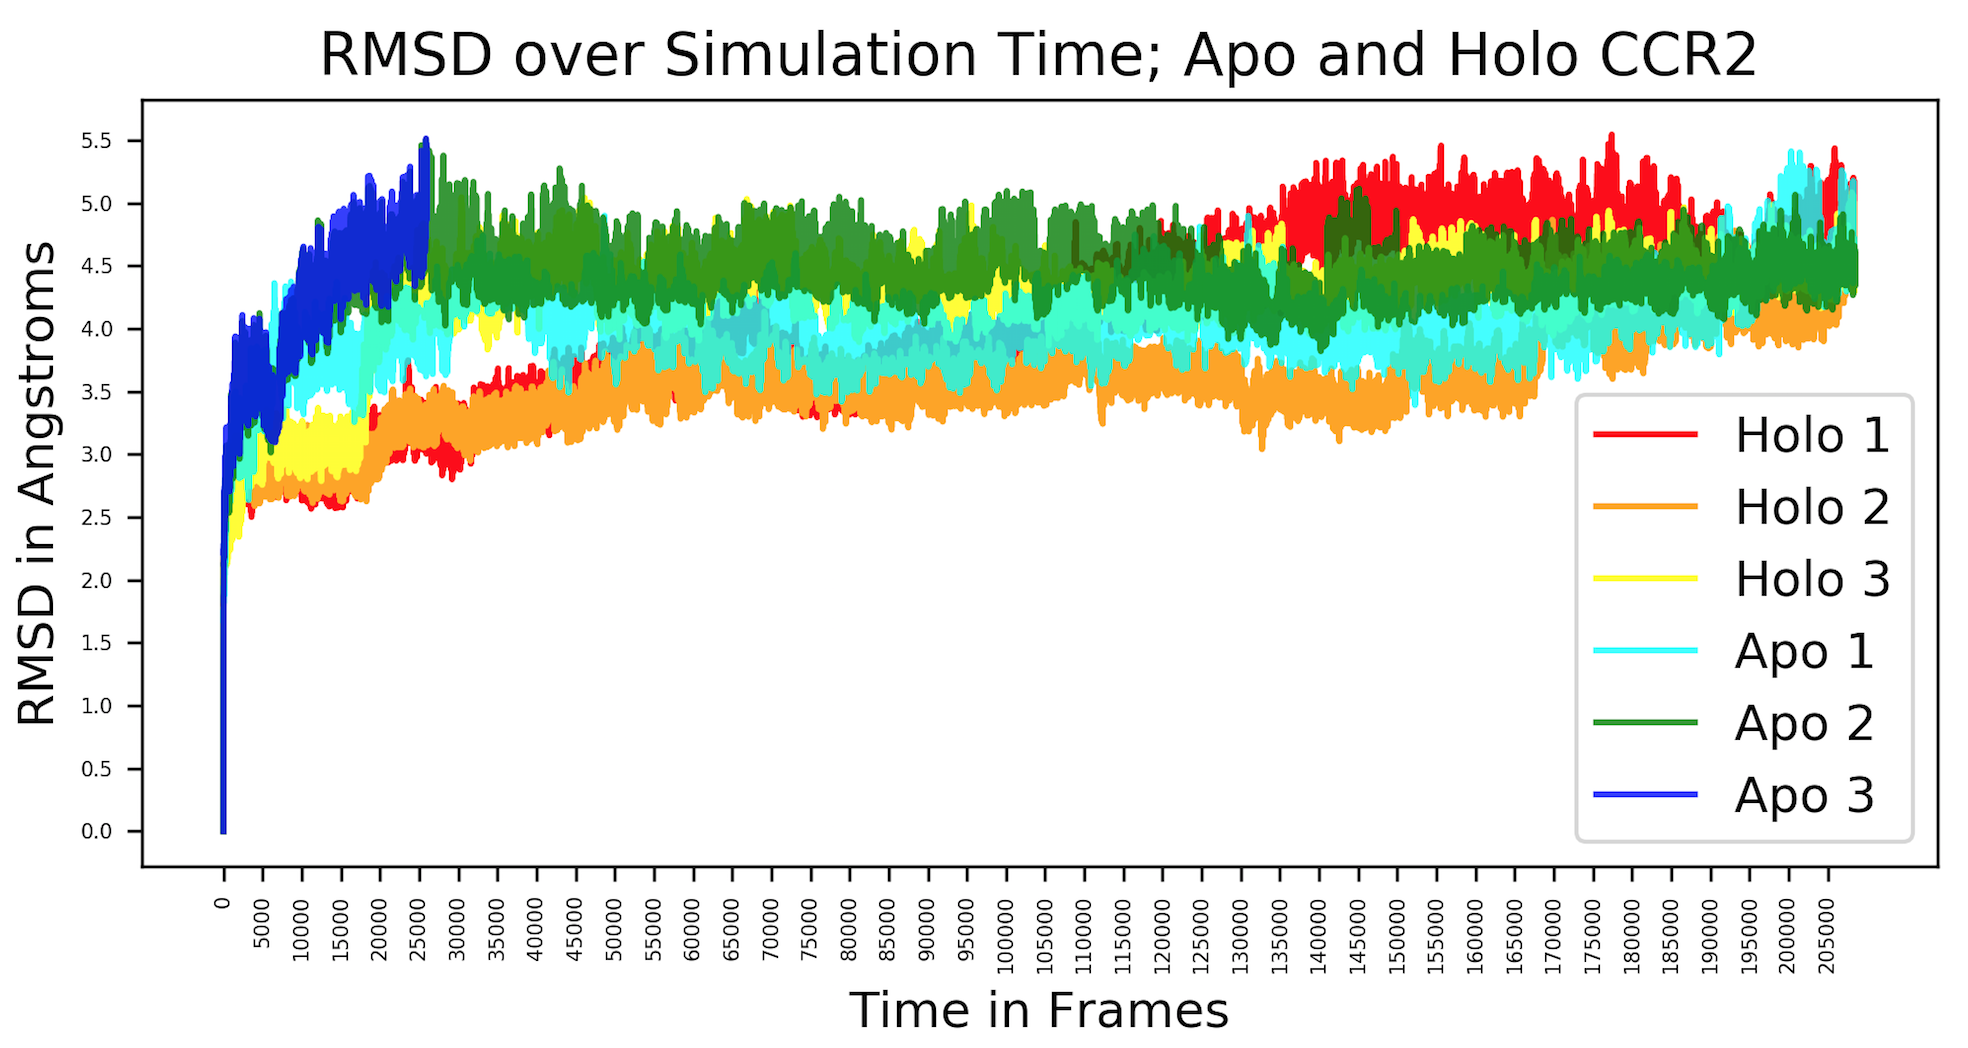
\includegraphics[width=\textwidth]{./figures/rmsd.png}
\caption{RMSD plot of all trajectories over simulation time.}
\label{fig:rmsd}
\end{figure}

% figure alloligand 2
\begin{figure}[htbp]
  \centering
  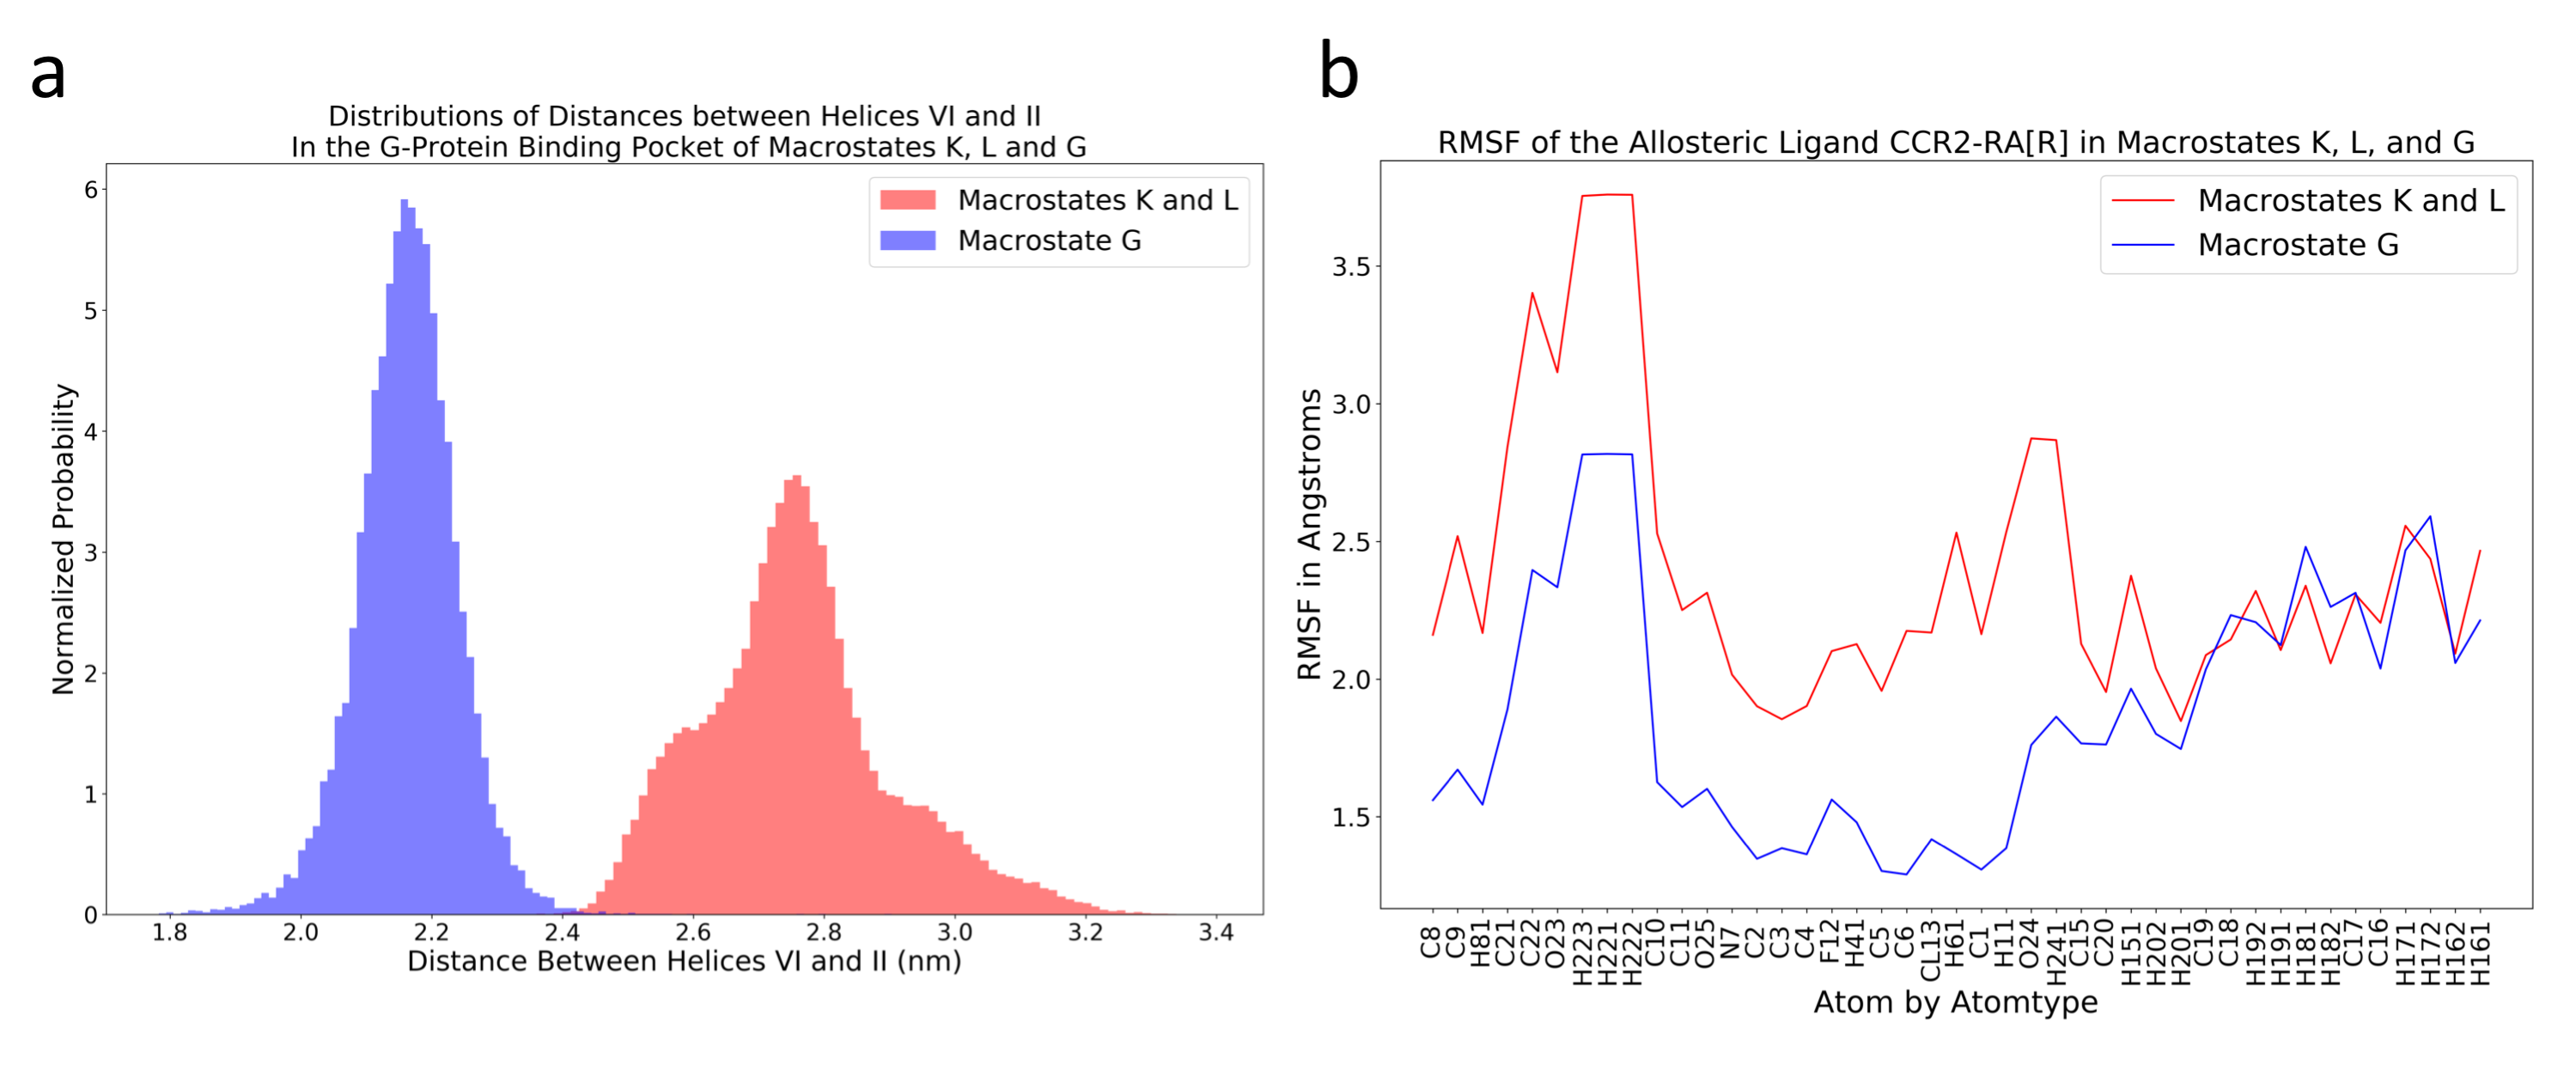
\includegraphics[width=\textwidth]{./figures/alloligand.png}
 \caption{The RMSF of the allosteric ligand is larger in macrostates with more open G-protein binding sites. A) Distribution of distances in macrostates K, L and G between residues Gly 224 and Asp 78 in the intracellular regions of helices VI and II. B) RMSF of the allosteric ligand in holo macrostates K, L, and G.}
  \label{fig:alloligand}
\end{figure}

%trp 256 3
\begin{figure}[htbp]
\centering
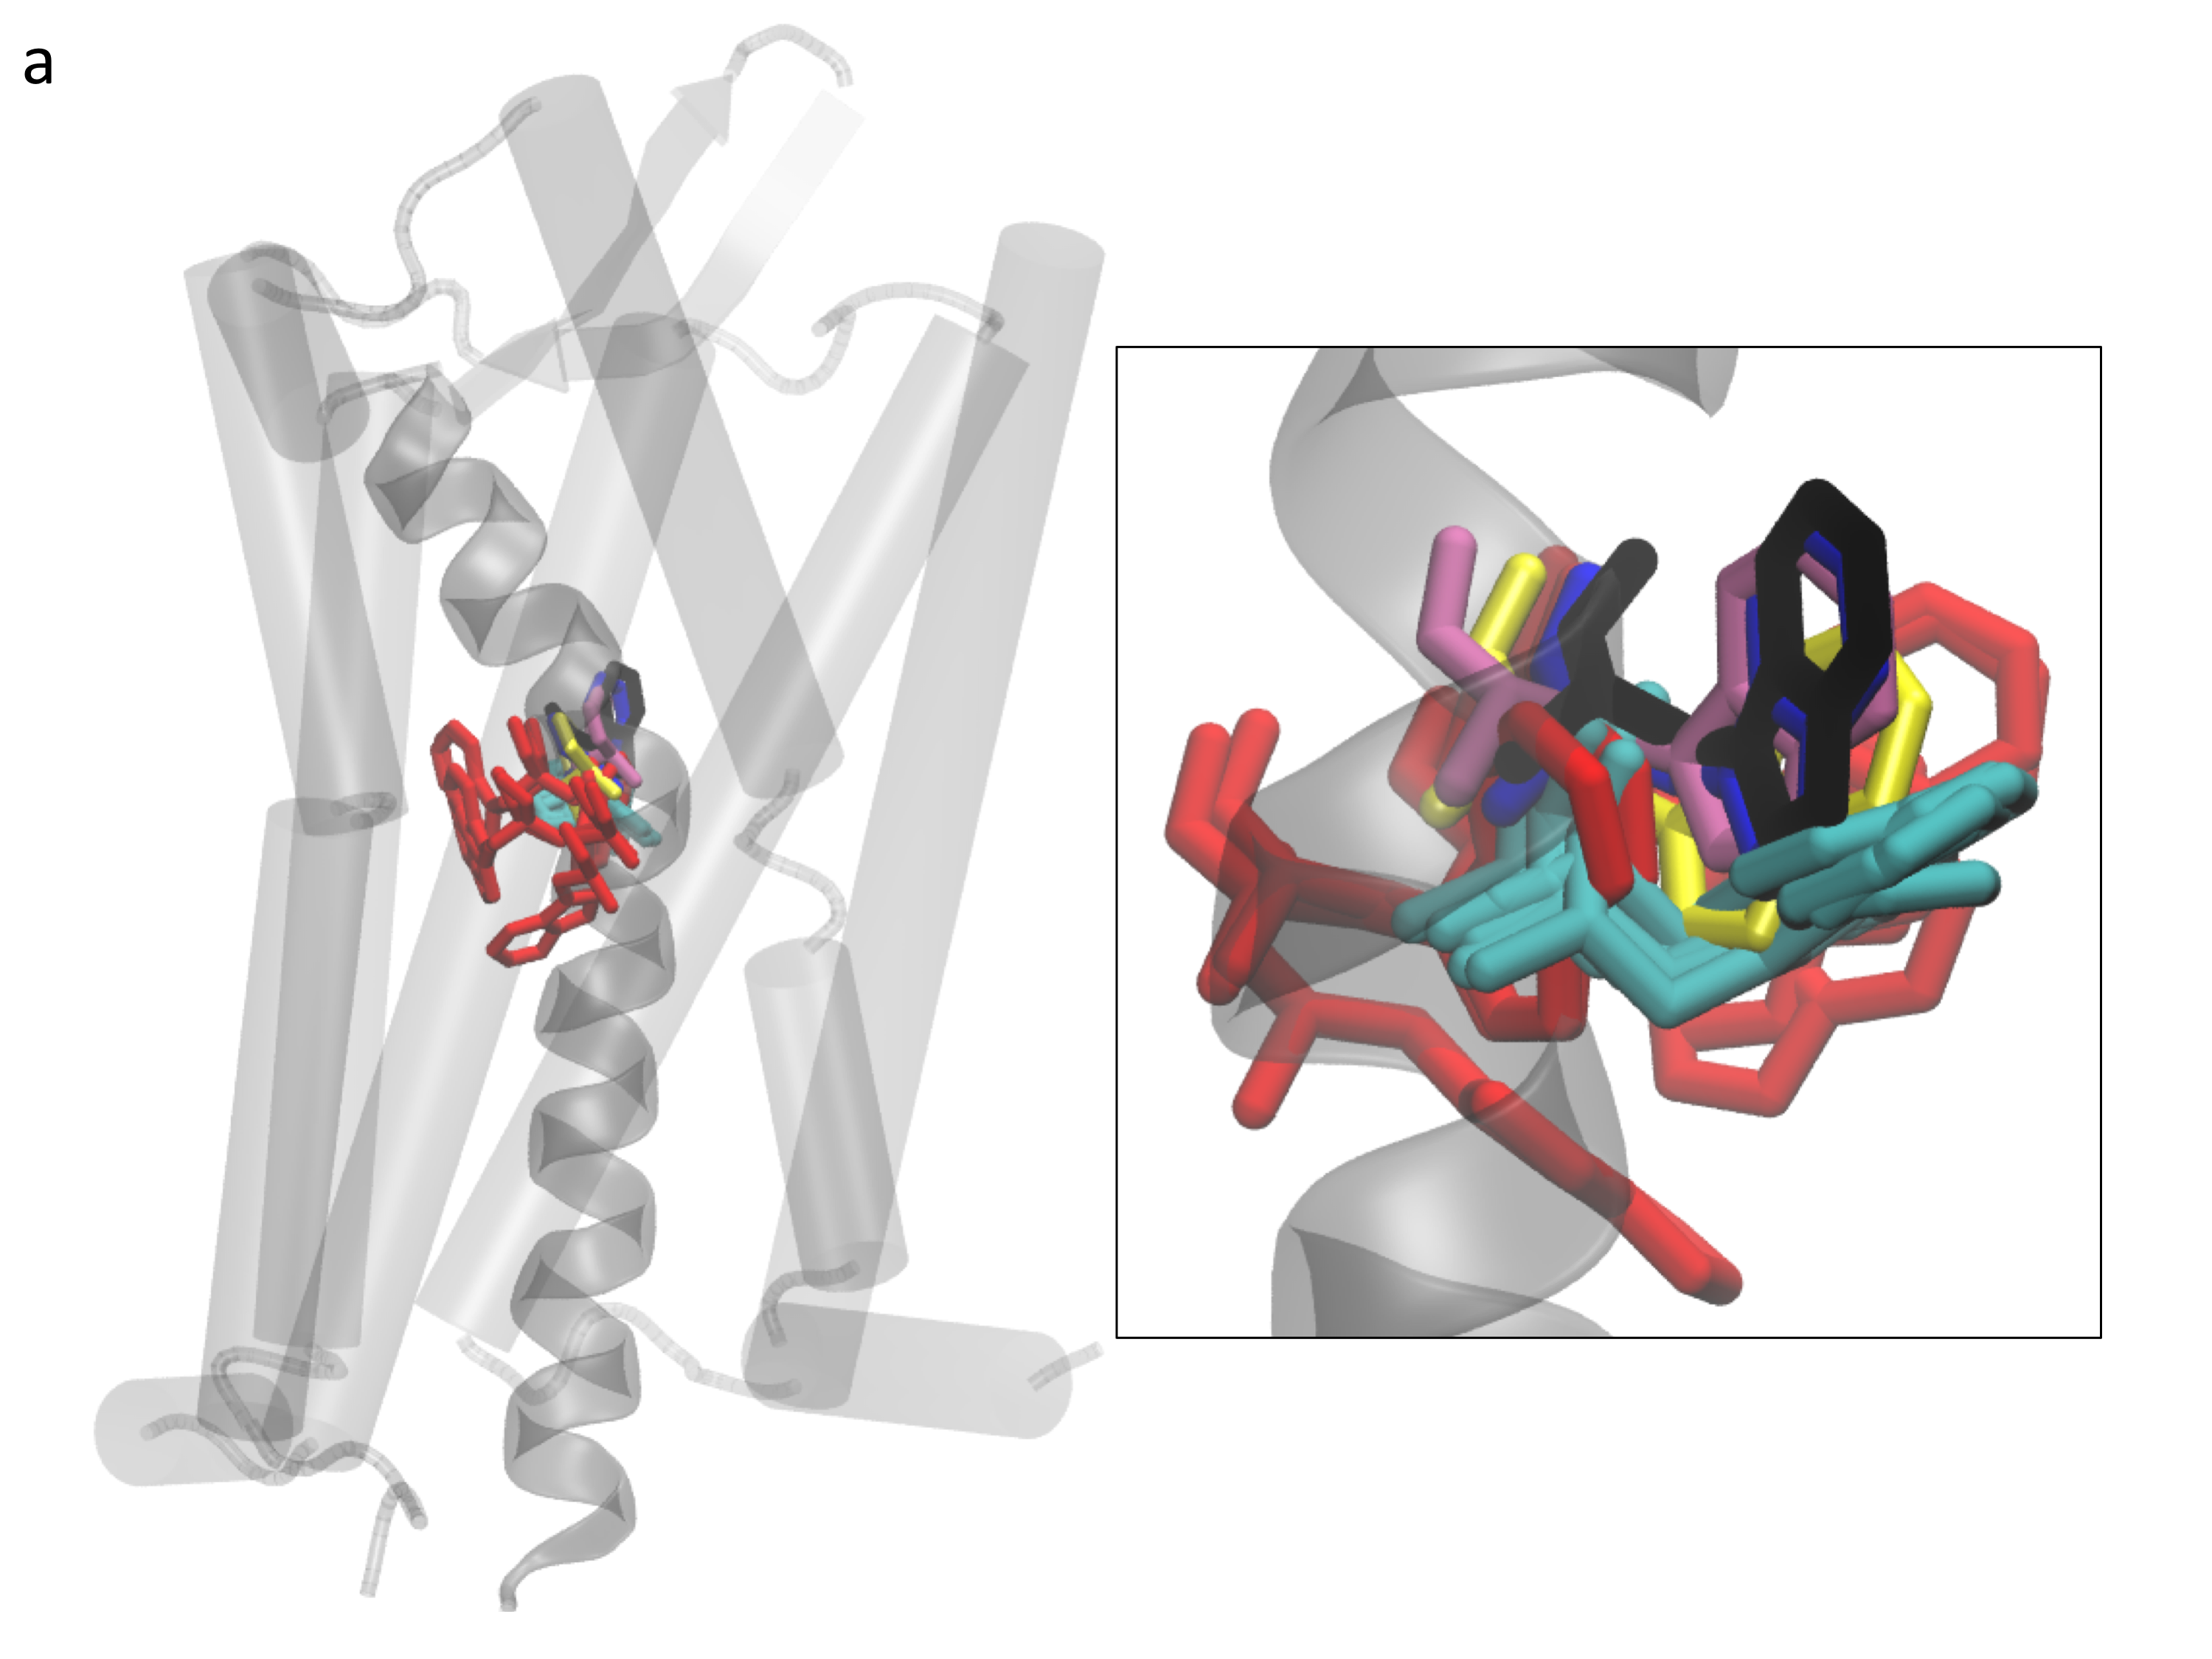
\includegraphics[width=\textwidth]{./figures/trp256.png}
\caption{Trp 256\textsuperscript{6.48} compared to the apo and holo macrostates and the crystal structures of CCR2 (PDB ID: 5T1A; grey, black) CCR5 (PDB ID: 4MBS; blue) and CXCR4 (PDB ID: 4RWS; mauve). A) Each apo macrostate shows Trp 256\textsuperscript{6.48} in a single conformation pointing toward helix III. In the holo macrostates, Trp 256\textsuperscript{6.48} access three distinct conformations: one resembling the crystal structure but with the helix shifted slightly outward from the helical core, another that laterally twists toward helix V, and one conformation that points down into the helical core toward the G-protein binding site.}
\label{fig:trp256}
\end{figure}

% Water, sodium 4
\begin{figure}[htbp]
\centering
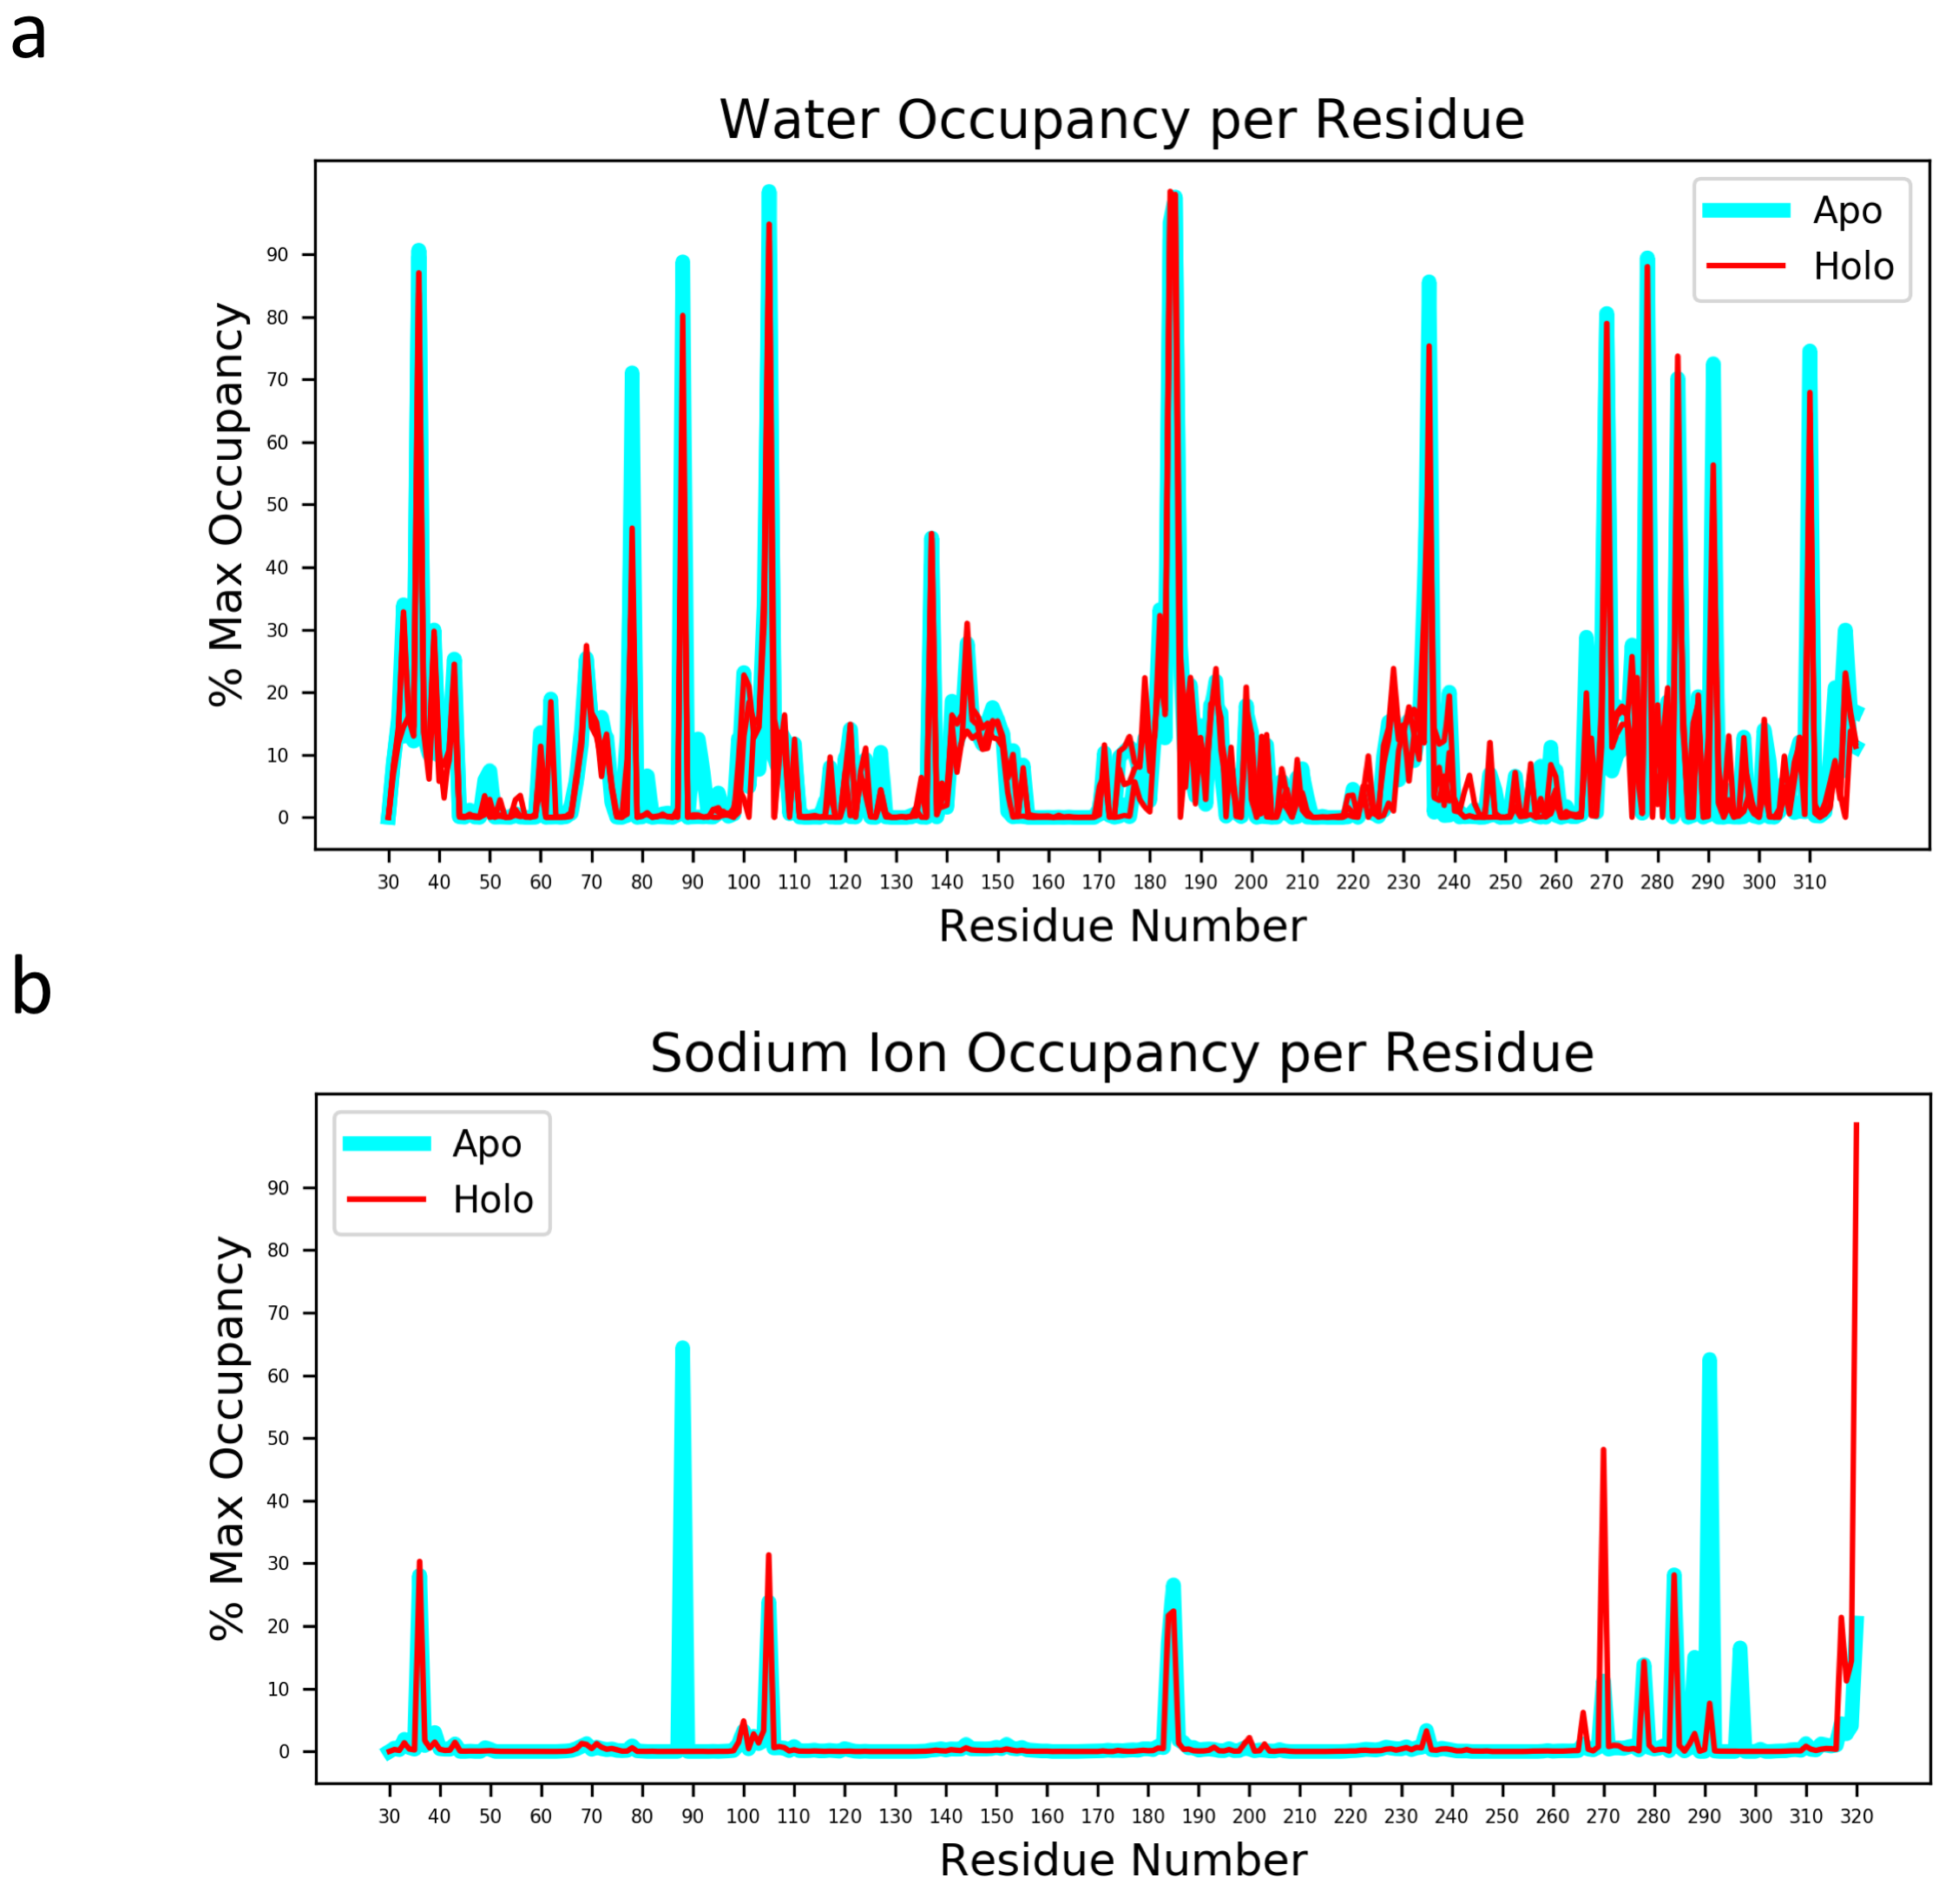
\includegraphics[width=\textwidth]{./figures/water_na_plots.png}
\caption{Ligands disrupt a continuous internal water and sodium ion pathway. A) Water occupancy per residue in all apo (teal) and holo (red) simulations. B) Sodium ion occupancy per residue in all apo and holo simulations.}
\label{fig:water_na_plots}
\end{figure}

% table S2
\begin{table}[htbp]
\centering
\begin{tabular}{|c|c|c|c|c|c|c|c|c|c|c|}
\hline
\textbf{Apo} & 321.6 $\mu$s & 57.7 $\mu$s & 11.1 $\mu$s & 9.0 $\mu$s & 4.2 $\mu$s & 2.8 $\mu$s & 2.4 $\mu$s & 1.7 $\mu$s & 1.3 $\mu$s & 1.3 $\mu$s\\ \hline
%\textbf{Apo} & 321.6 & 57.7 & 11.1 & 9.0 & 4.2 & 2.8 & 2.4 & 1.7 & 1.3 & 1.3 \\ \hline
\textbf{Holo} & 2246.9 $\mu$s & 286.8 $\mu$s & 84.9 $\mu$s & 59.1 $\mu$s & 44.3 $\mu$s & 21.6 $\mu$s & 8.2 $\mu$s & 7.7 $\mu$s & 4.4 $\mu$s & 3.9 $\mu$s \\ \hline
%Holo & 2246.9 & 286.8 & 84.9 & 59.1 & 44.3 & 21.6 & 8.2 & 7.7 & 4.4 & 3.9 \\ \hline
\end{tabular}
\caption{Relaxation timescales for the apo and holo MSMs. Units are in microseconds.}
\label{table:relaxation_timescales}
\end{table}

% tics 5
\begin{figure}[htbp]
  \begin{center}
  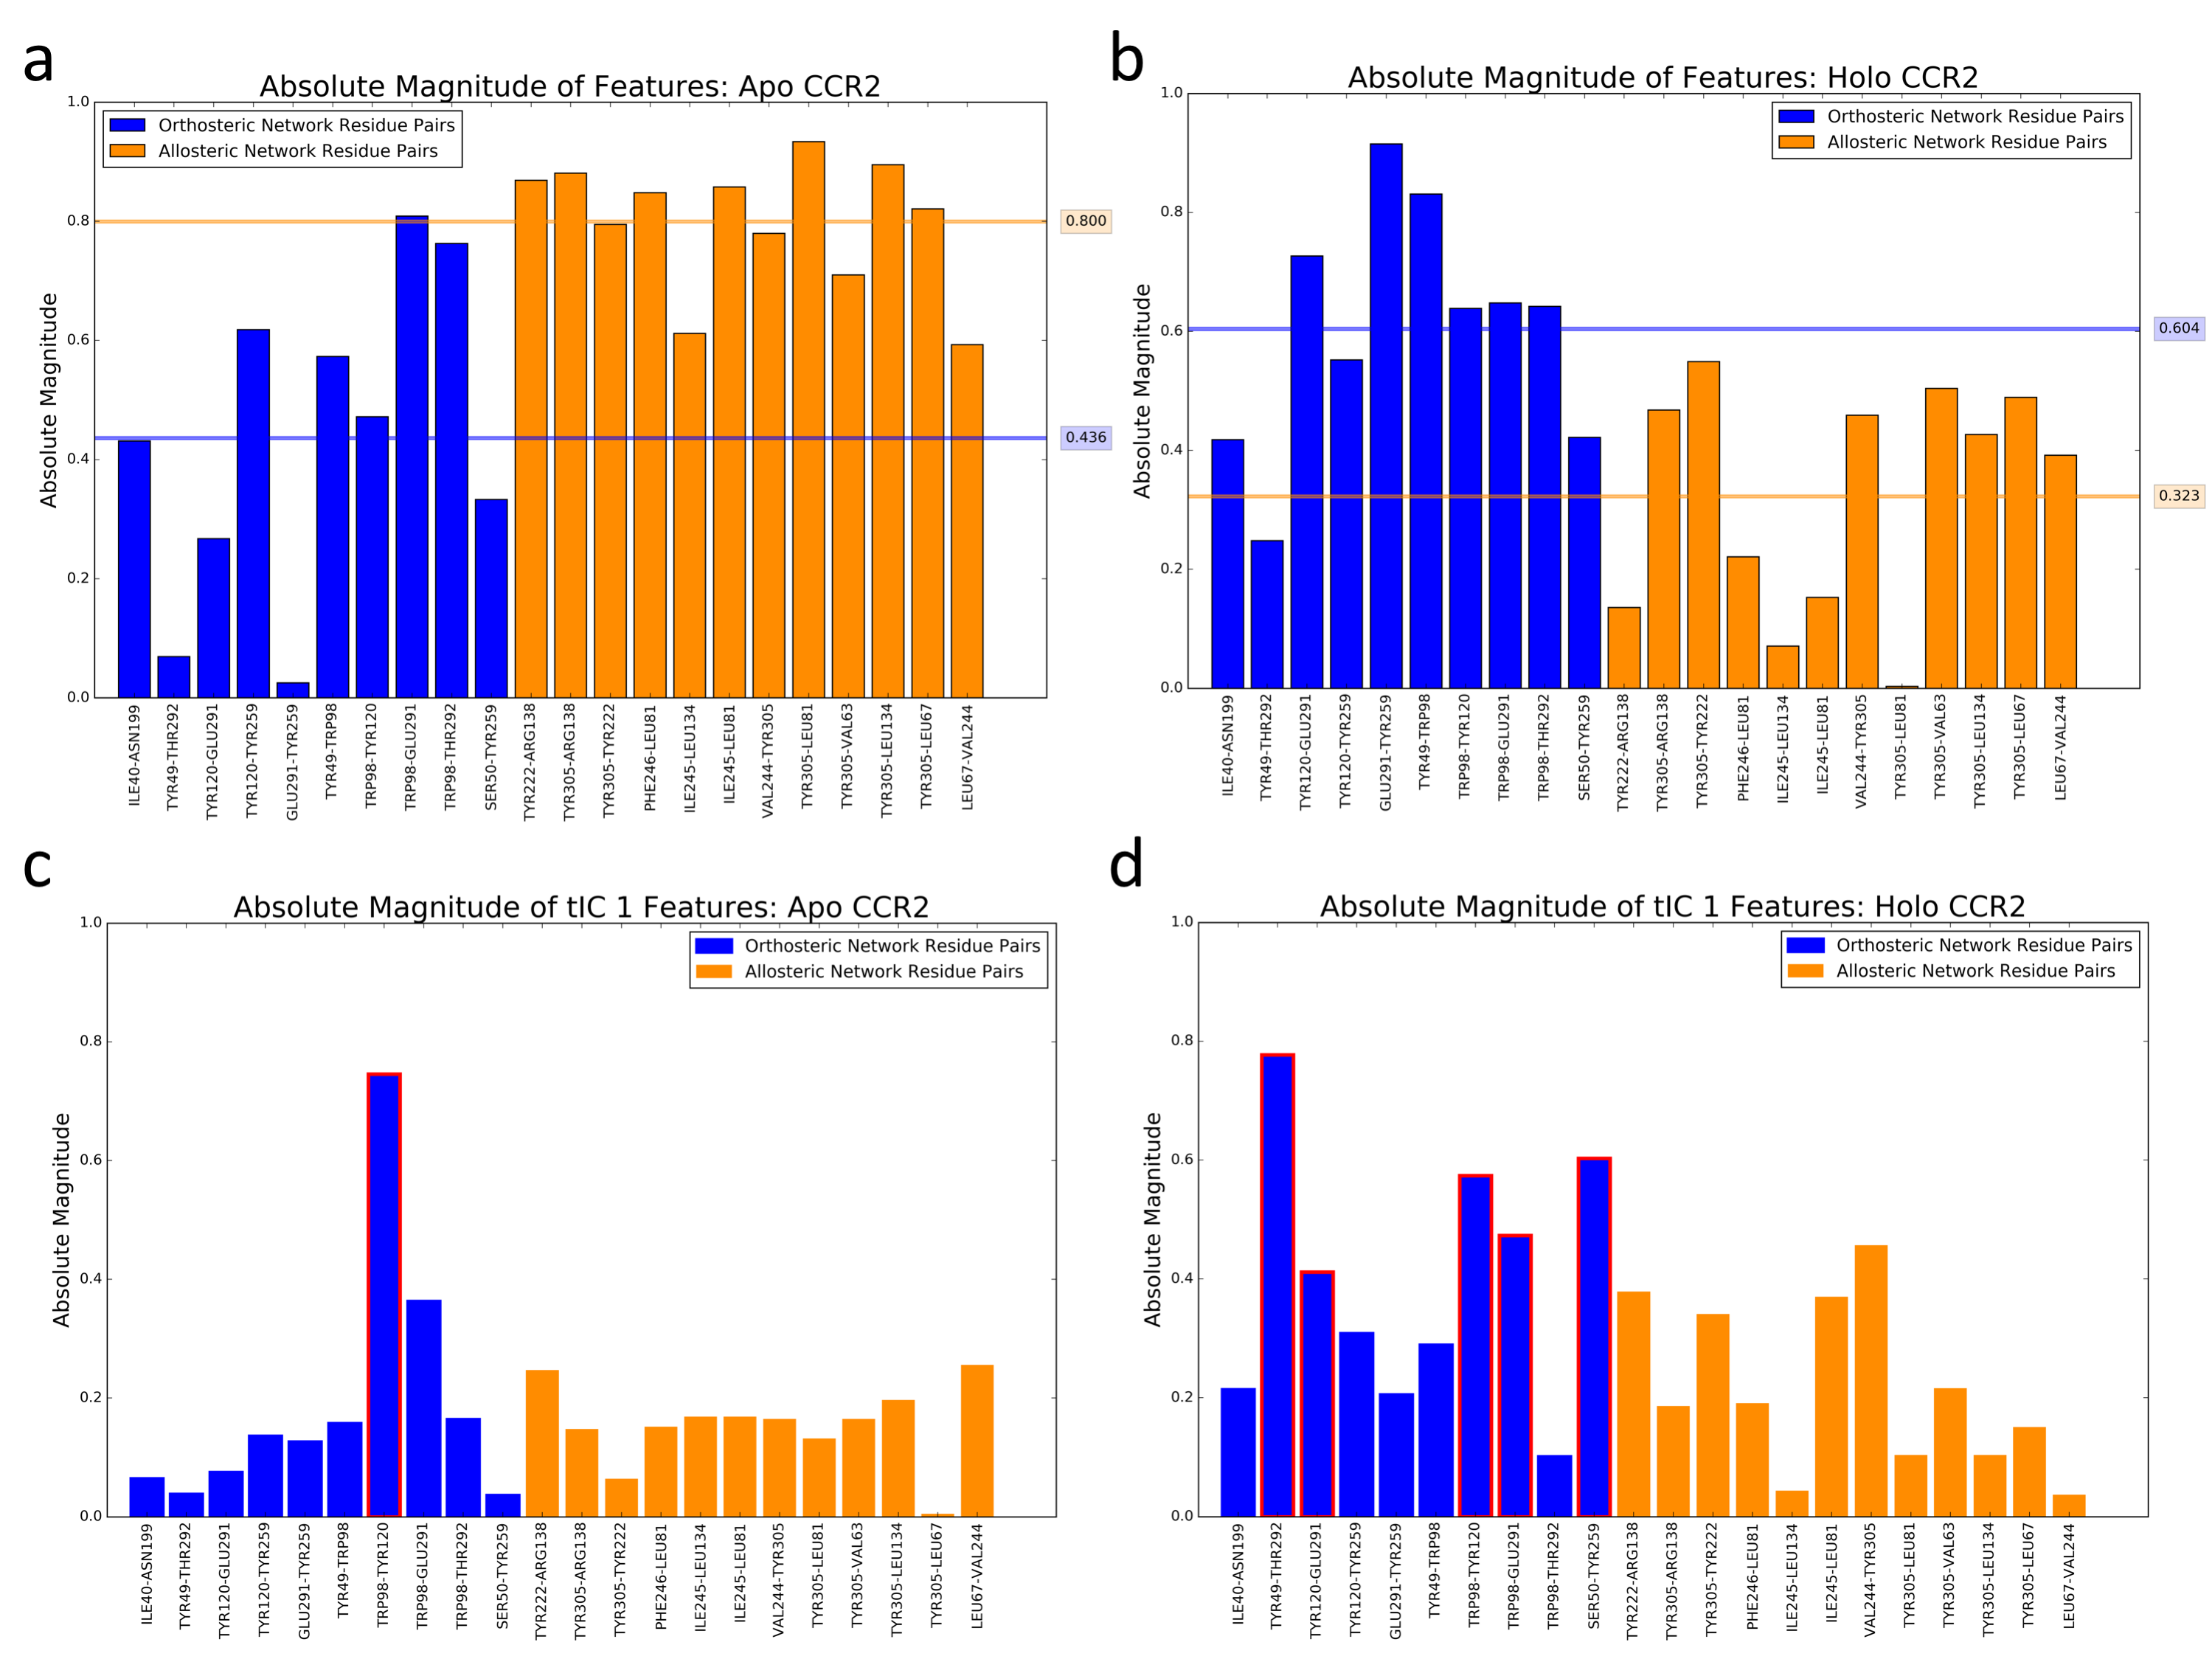
\includegraphics[width=\textwidth]{./figures/tic0_tic1_contributions.png}
\caption{The absolute magnitude of each input feature in A) apo TIC 0, B) holo TIC 0, C) apo TIC 1, and D) holo TIC 1. Each bar represents the absolute magnitude of one inter-residue distance. Blue bars are distances between residue pairs in the orthosteric pocket, and orange bars are distances between residue pairs in the allosteric pocket.}
\label{fig:tic0_contributions}
  \end{center}
\end{figure}

% apo F 6
\begin{figure}[htbp]
\centering
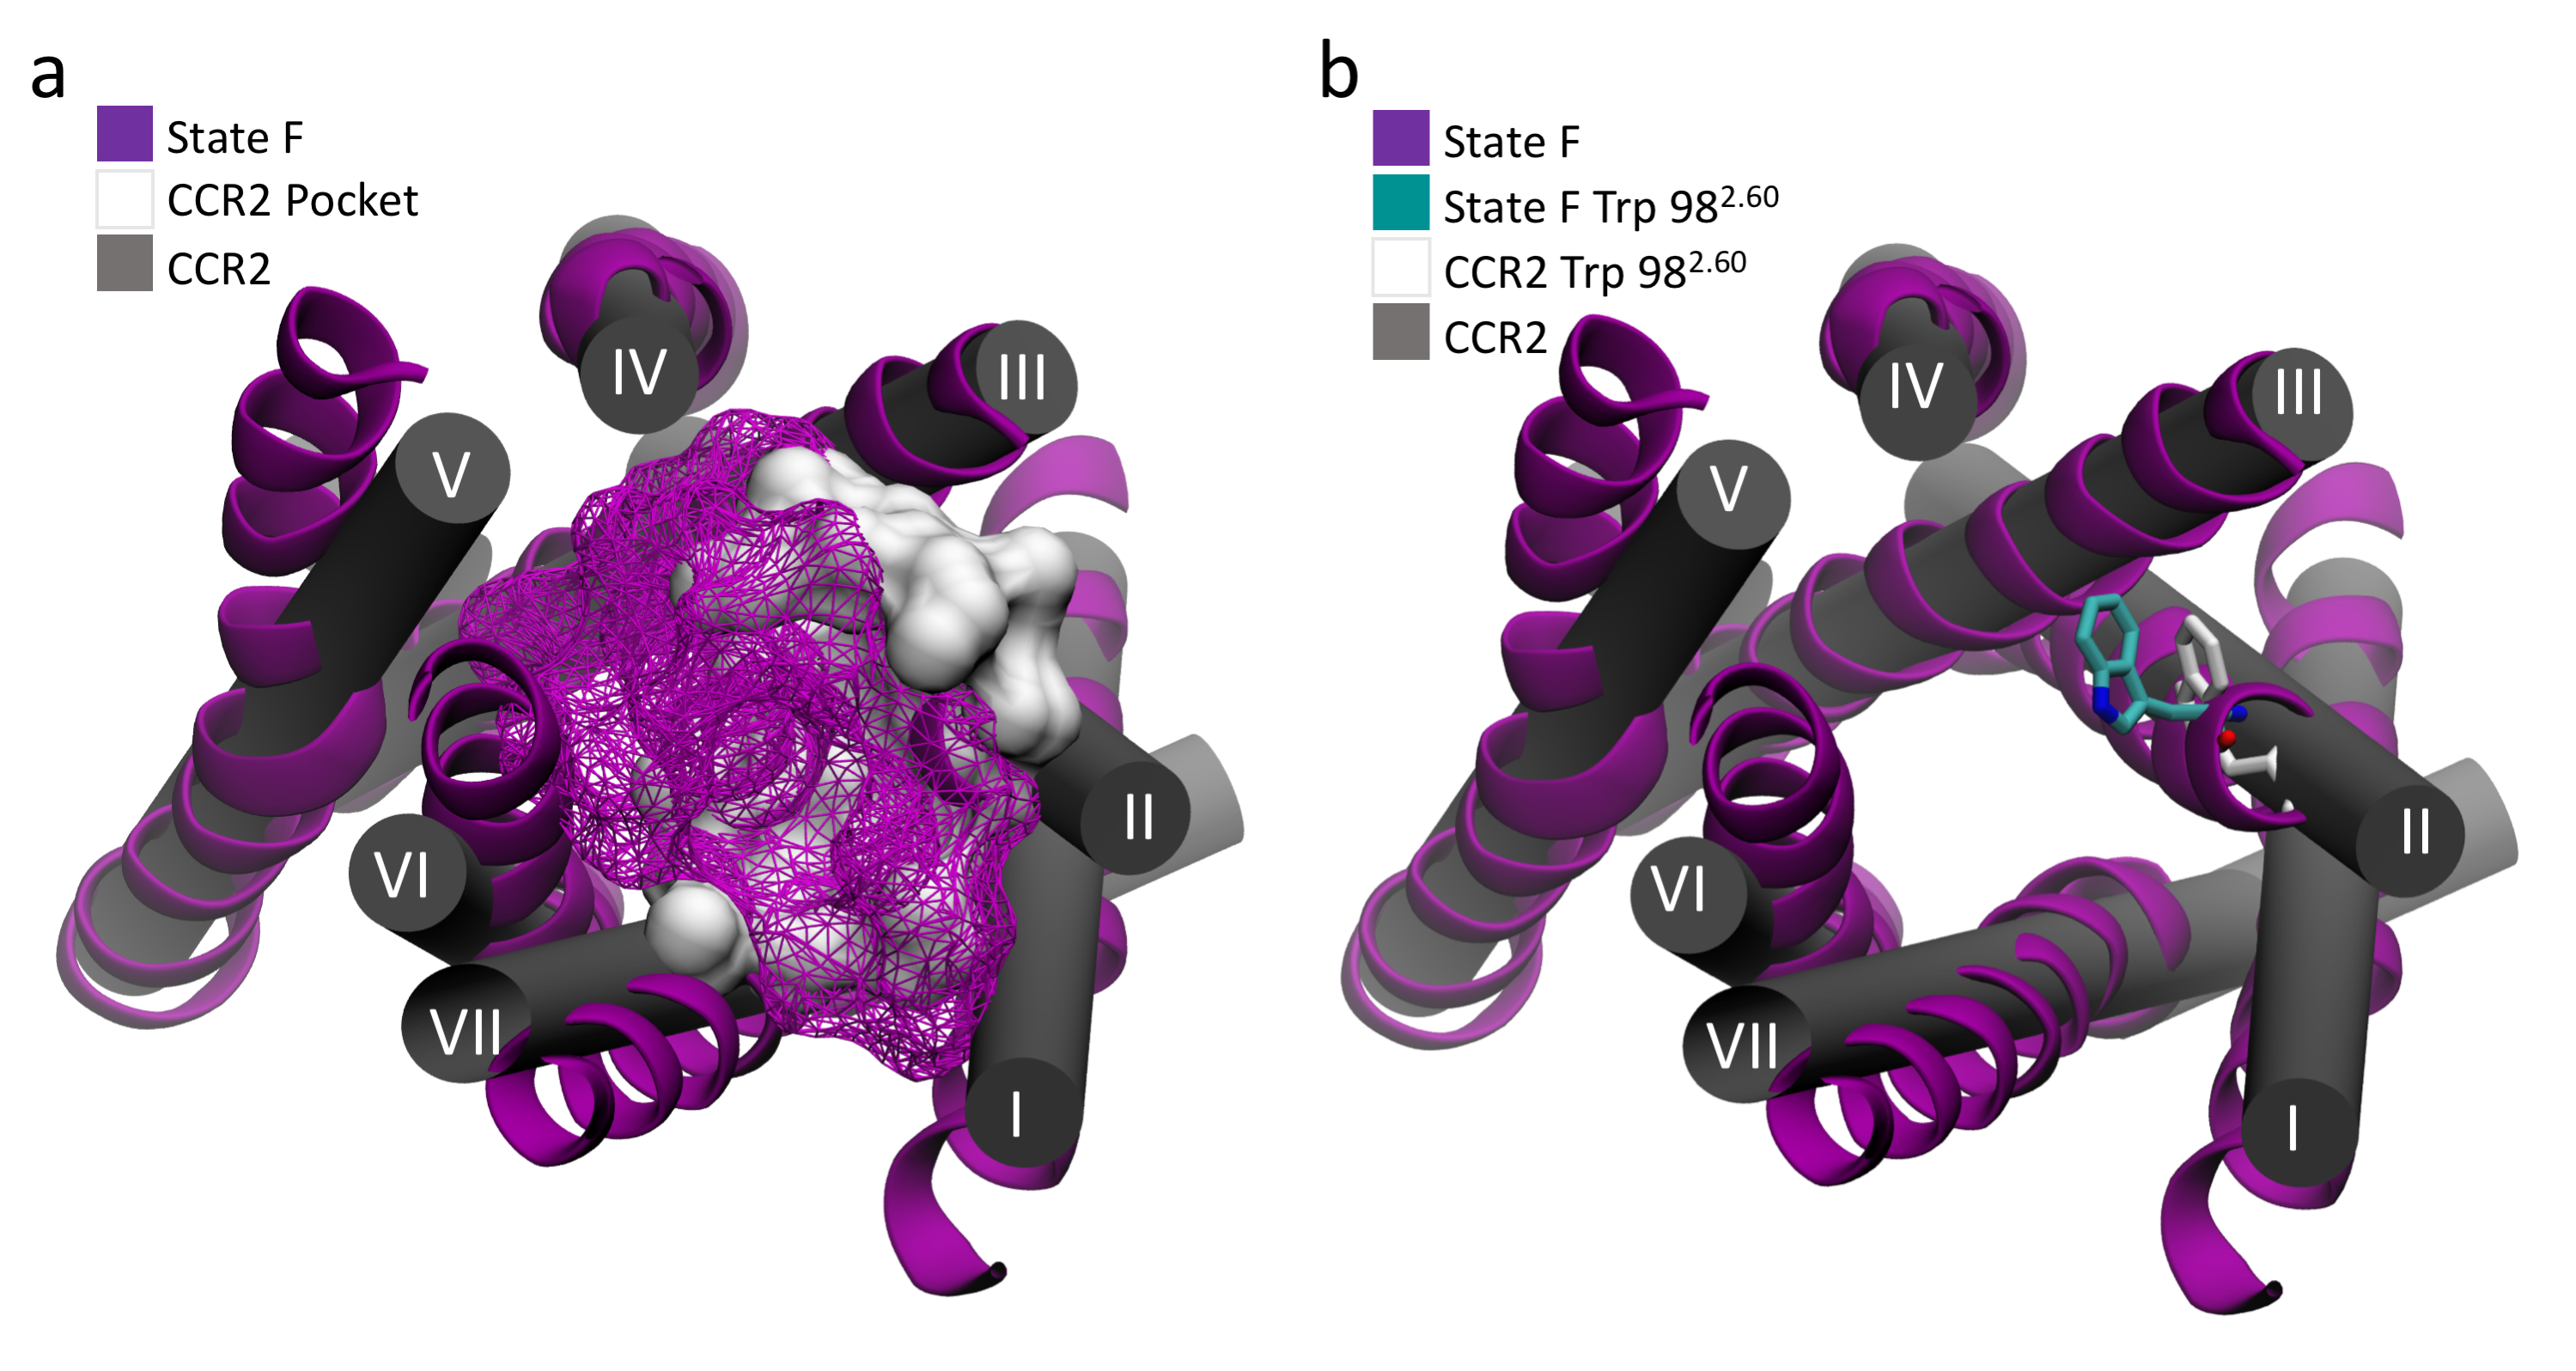
\includegraphics[width=\textwidth]{./figures/apoF_ccr2_orthopocketSI.png}
\caption{A) The shape of the chemokine binding site of apo state F in comparison to the crystal structure. Without the ligand, the binding site expands and rotates toward helices IV,  V,  and VI, and extends between helices I and VII. B) The conformations of Trp98\textsuperscript{2.60} in apo state F and the crystal structure. Trp98\textsuperscript{2.60} protrudes into the pocket in the absence of ligands.}
\label{fig:apoF_ccr2_orthopocketSI}
\end{figure}

% tic 1 7
\begin{figure}
\centering
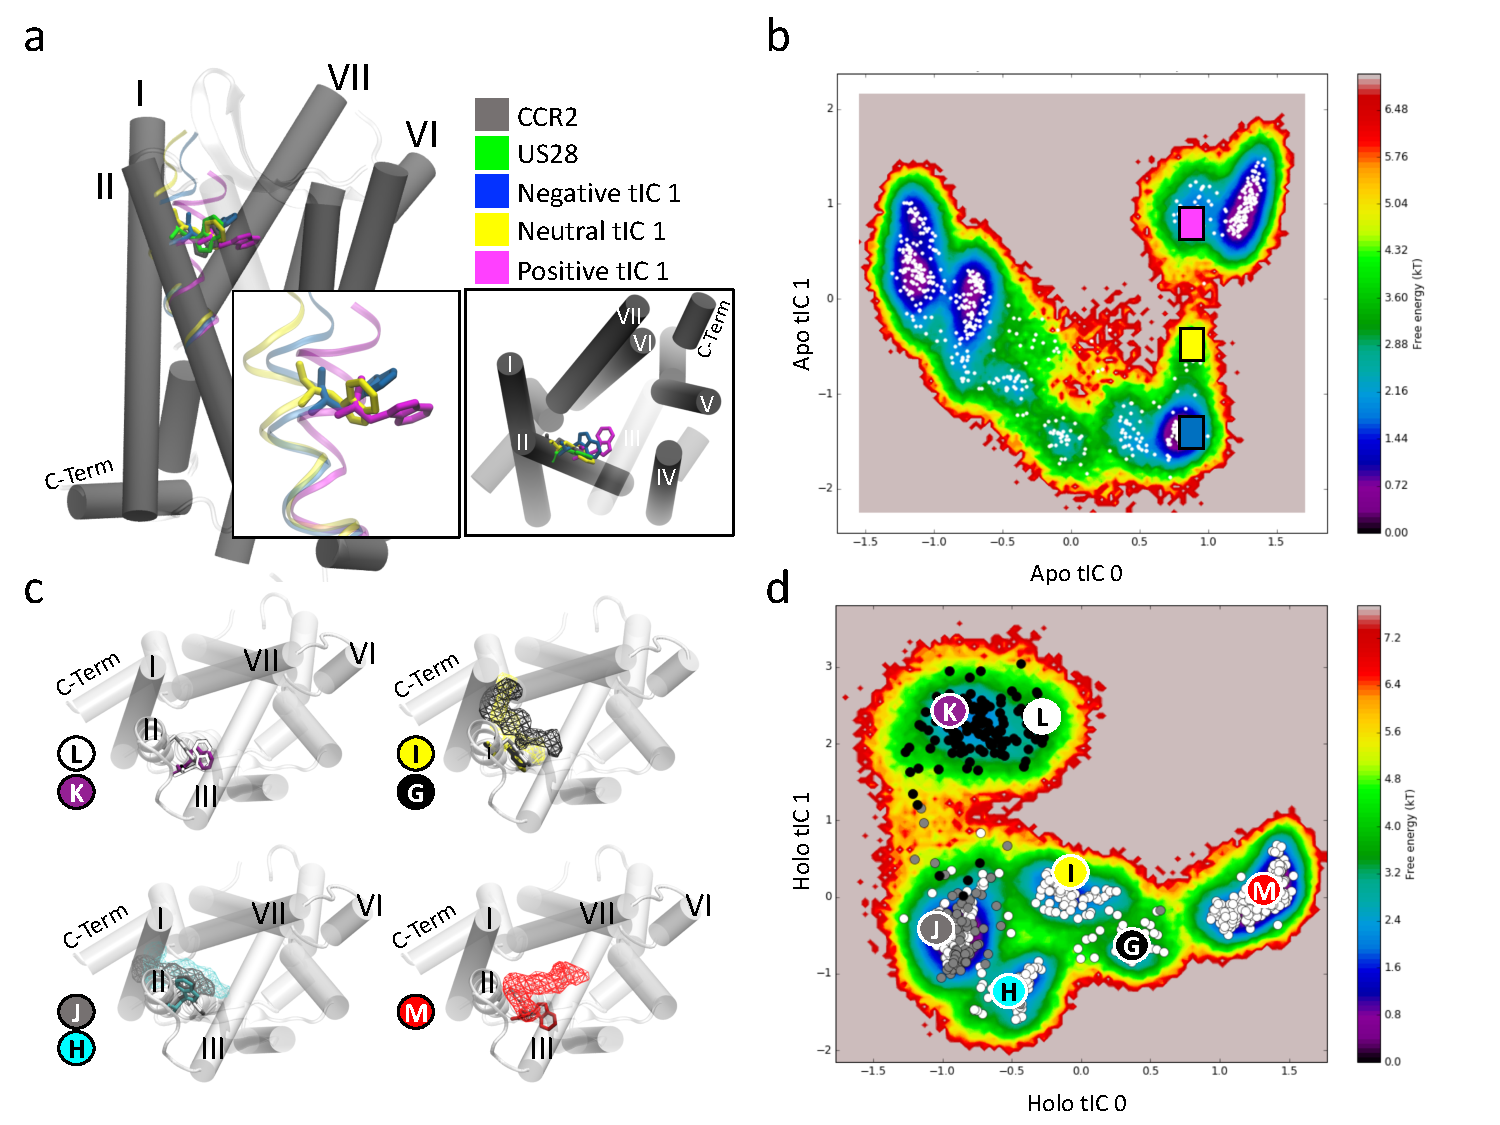
\includegraphics[width=\textwidth]{./figures/tic1_trp98_apo_holo.pdf}
\caption{A) In apo CCR2, TIC 1 represents Trp 98\textsuperscript{2.60} in three distinct positions. In gray is the crystal structure; in green is the active crystal structure of US28; in blue and yellow are transitions, and in magenta is the most dramatic conformation. Each conformation is plotted on the free energy in TICA space in B). C) In holo CCR2, the positioning of the orthosteric ligand and the conformation of Trp 98\textsuperscript{2.60} is closely linked. Shown in light silver cartoon is CCR2 5T1A; Trp 98\textsuperscript{2.60} is displayed as purple in state K, white in state L, gray in state J, cyan in state H, yellow in state I, black in state G, and red in state M. D) Holo CCR2. White circles are clusters of frames before any ligand dissociation. Grey circles are clusters of frames during the event. Black circles are clusters of frames after the event.}
\label{fig:tic1}
\end{figure}

% trp 98 centroids 8
\begin{figure}[htbp]
\centering
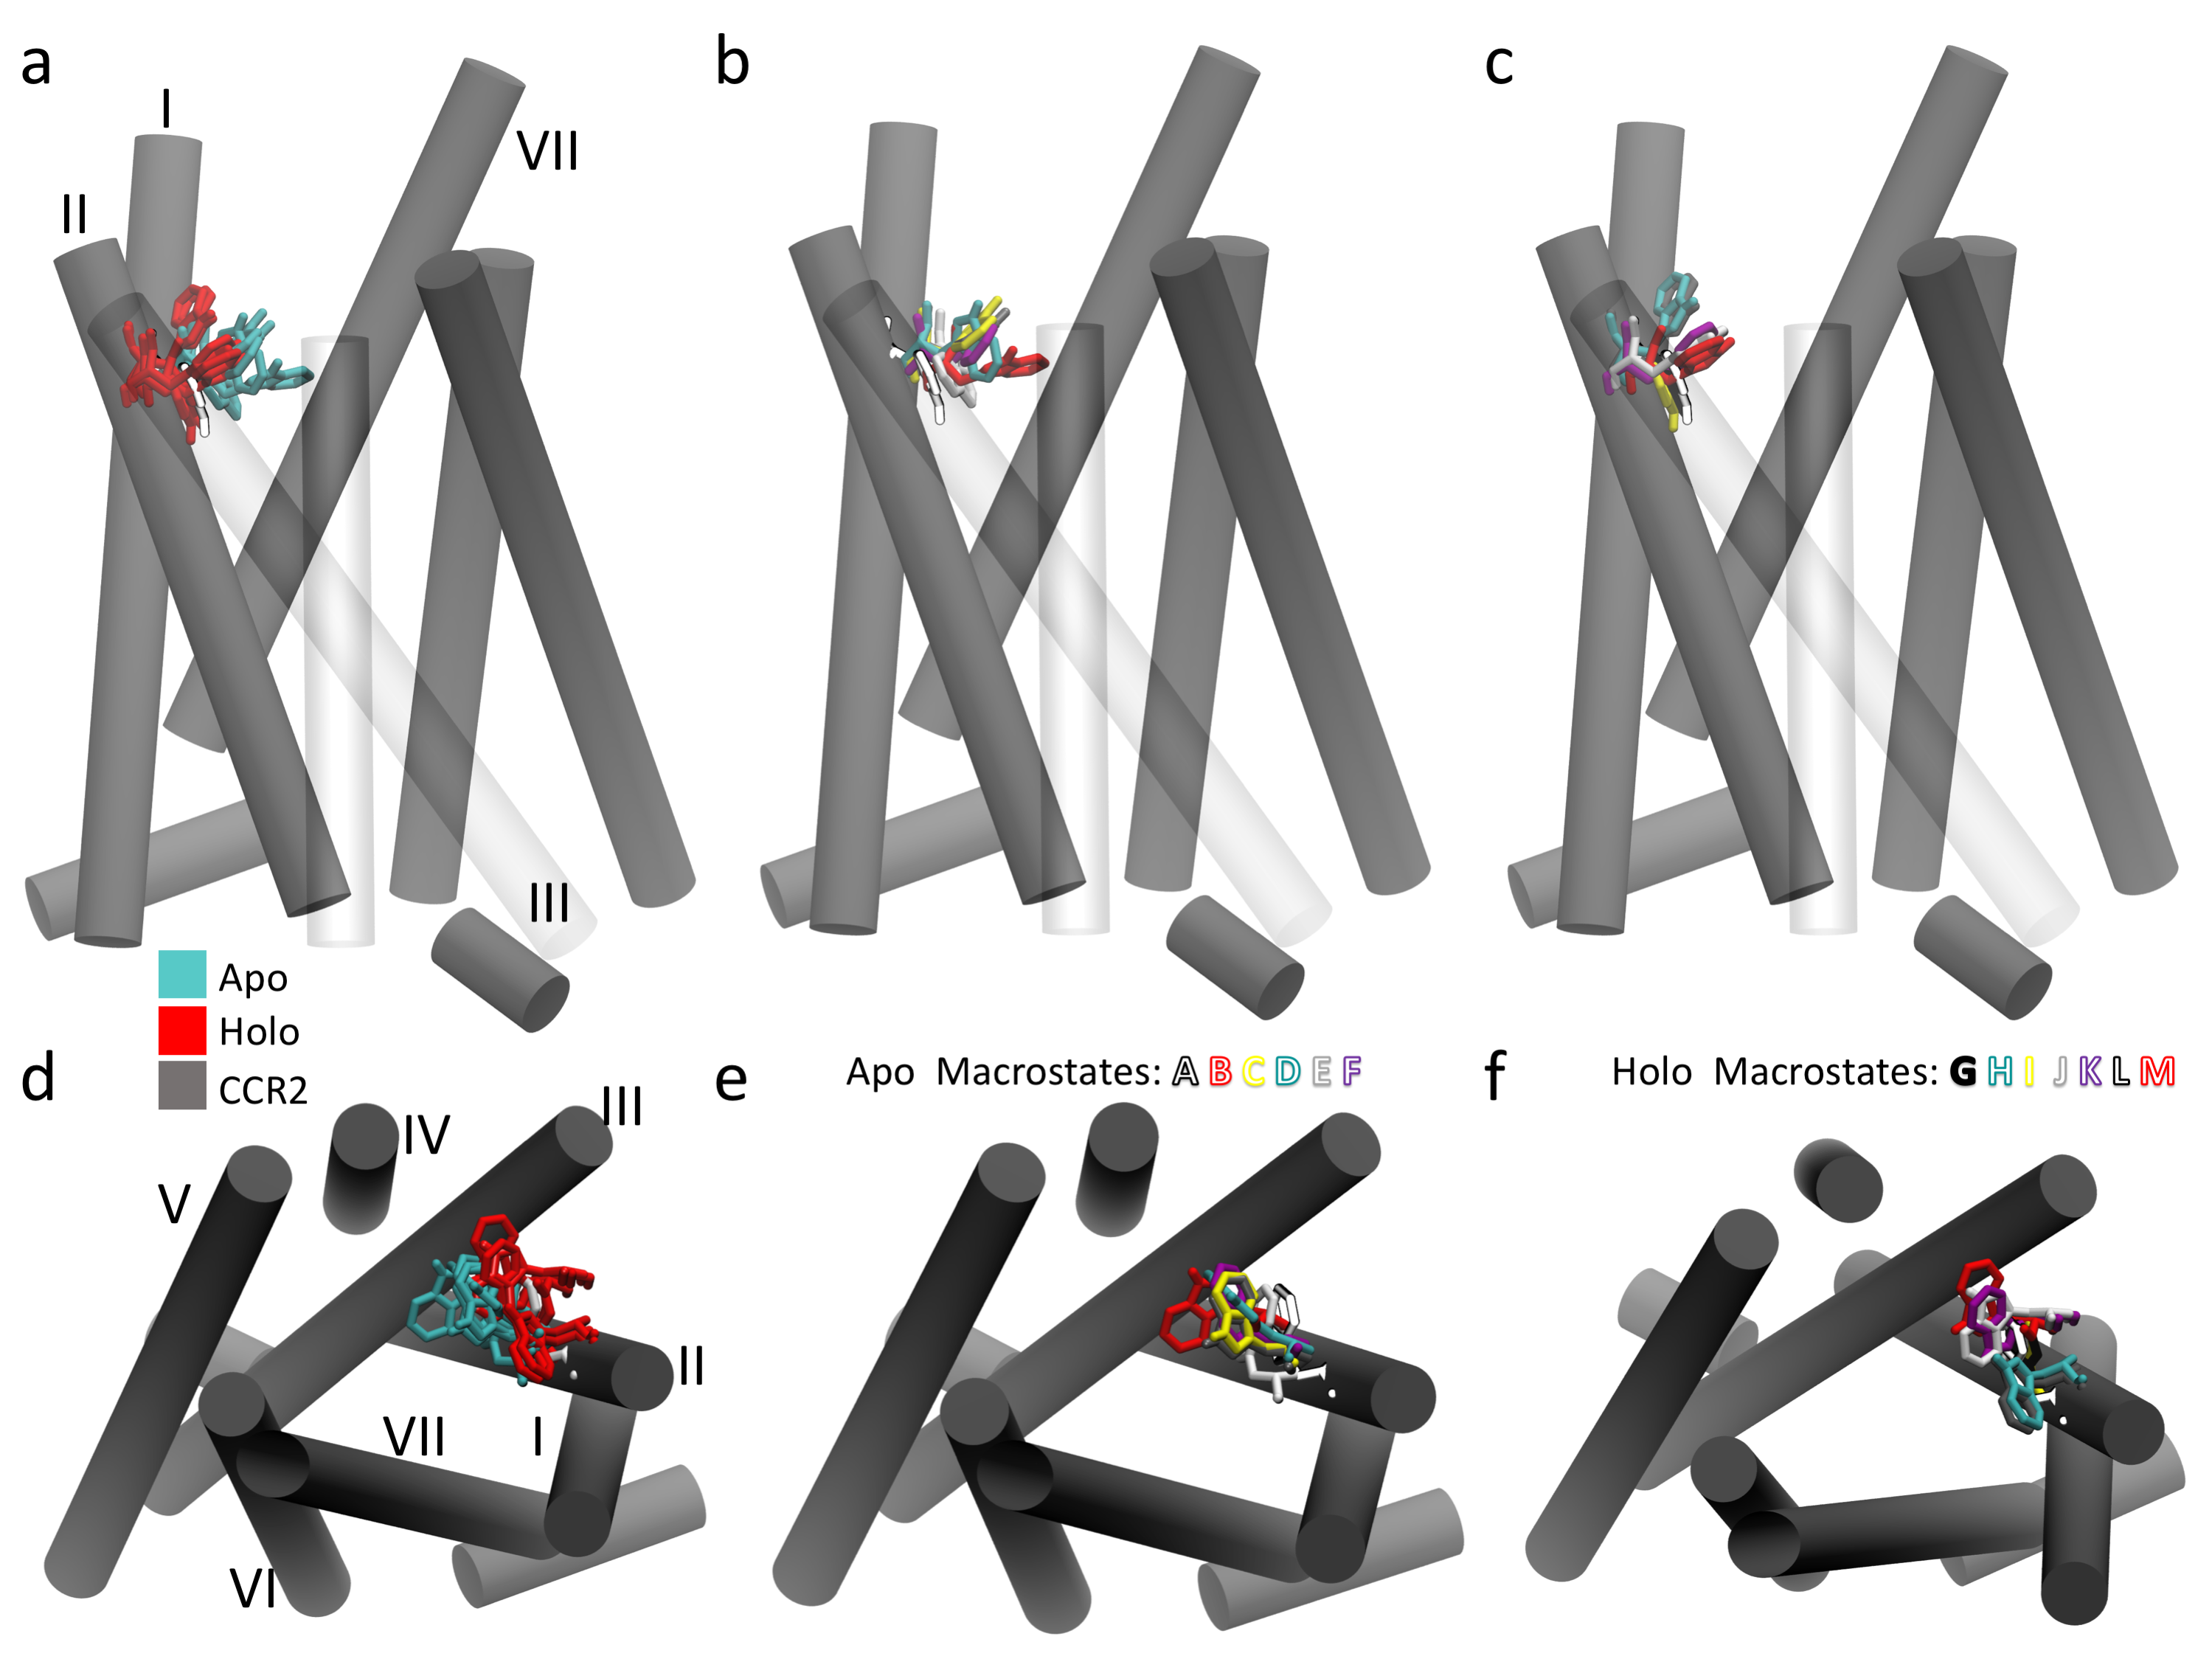
\includegraphics[width=\textwidth]{./figures/trp98_allcentroidsSI.png}
\caption{Trp 98\textsuperscript{2.60} extends farther into the chemokine binding site in apo CCR2 than in the holo crystal structure and holo macrostates. A side view of the CCR2 crystal structure (grey) and Trp 98\textsuperscript{2.60} (bright white) compared to A) the apo (cyan) and holo (red) macrostate conformations of Trp 98\textsuperscript{2.60}  B) the holo conformations, and C) the apo conformations. The extracellular-to-intracellular view of A)-C).}
\label{fig:trp98_allcentroidsSI}
\end{figure}


% trp 98 compared to ccr9  9
\begin{figure}[htbp]
\centering
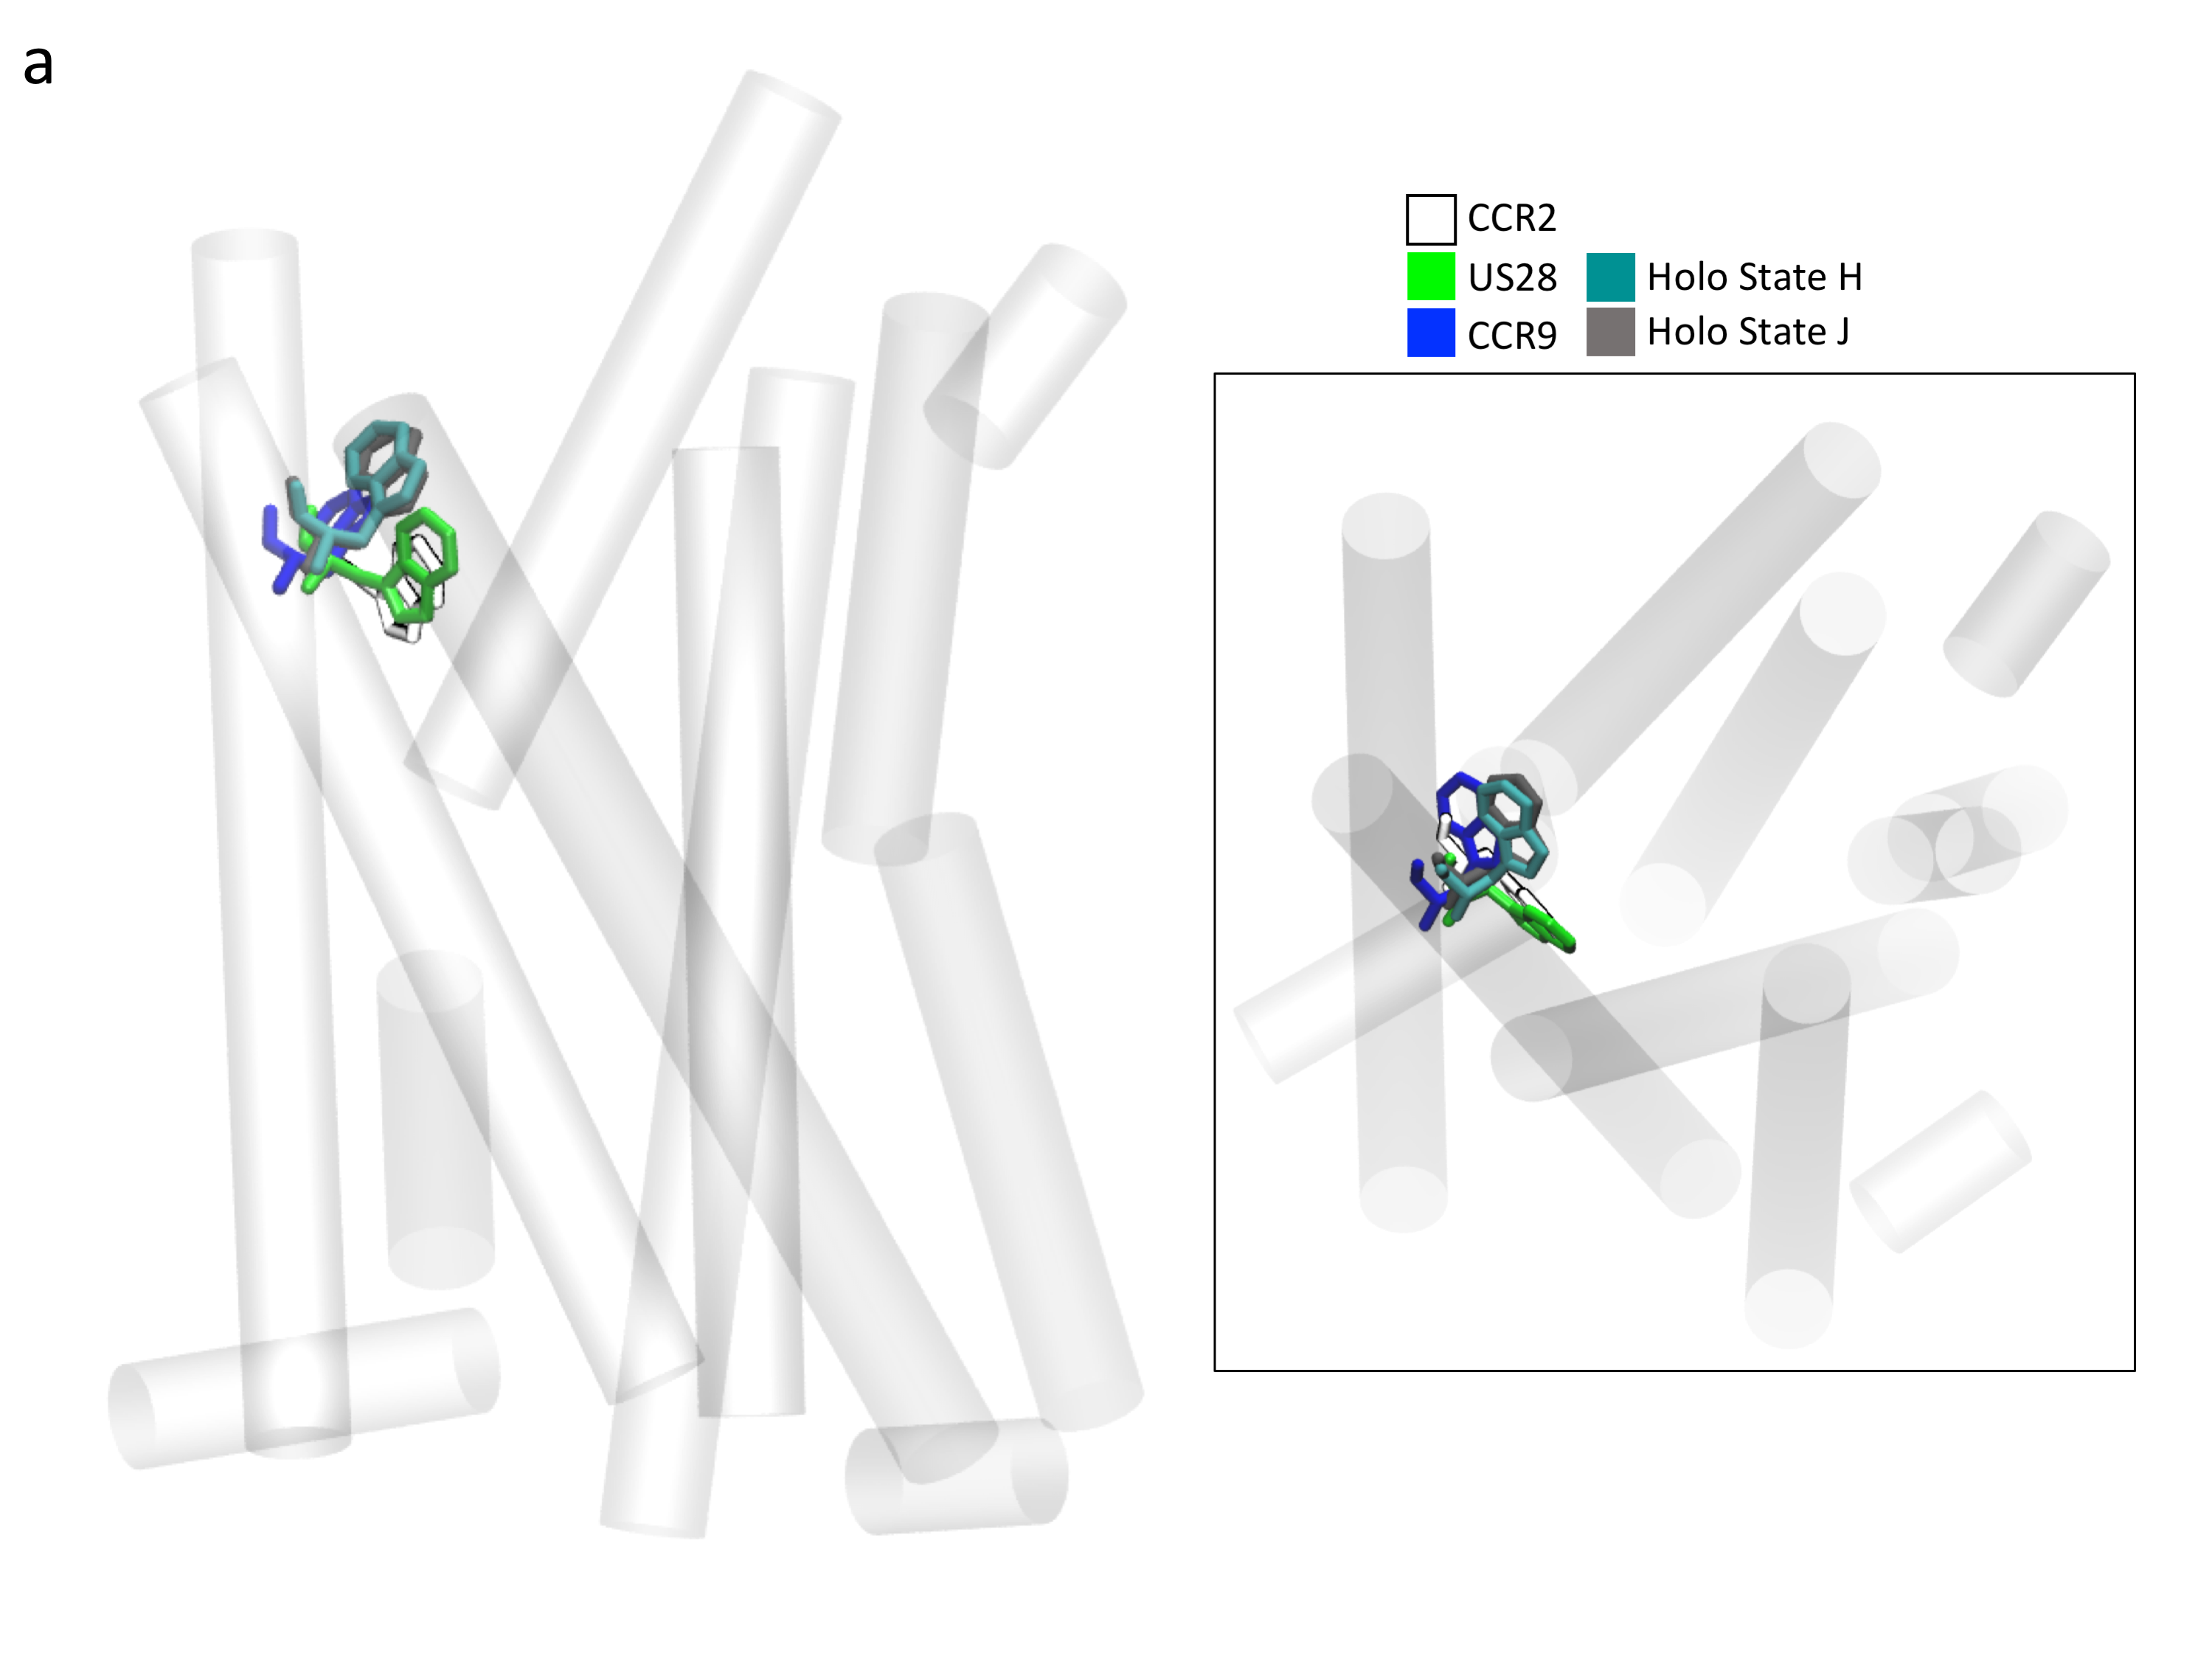
\includegraphics[width=\textwidth]{./figures/trp98_ccr9.png}
\caption{A) Trp 98\textsuperscript{2.60} in holo states H and J (cyan and grey) compared to CCR9 (dark blue) and the CCR2 crystal structure (white). Inset depicts the extracellular-to-intracellular view of A).}
\label{fig:trp98_ccr9}
\end{figure}


% 98-120 10
\begin{figure}[htbp]
  \centering
  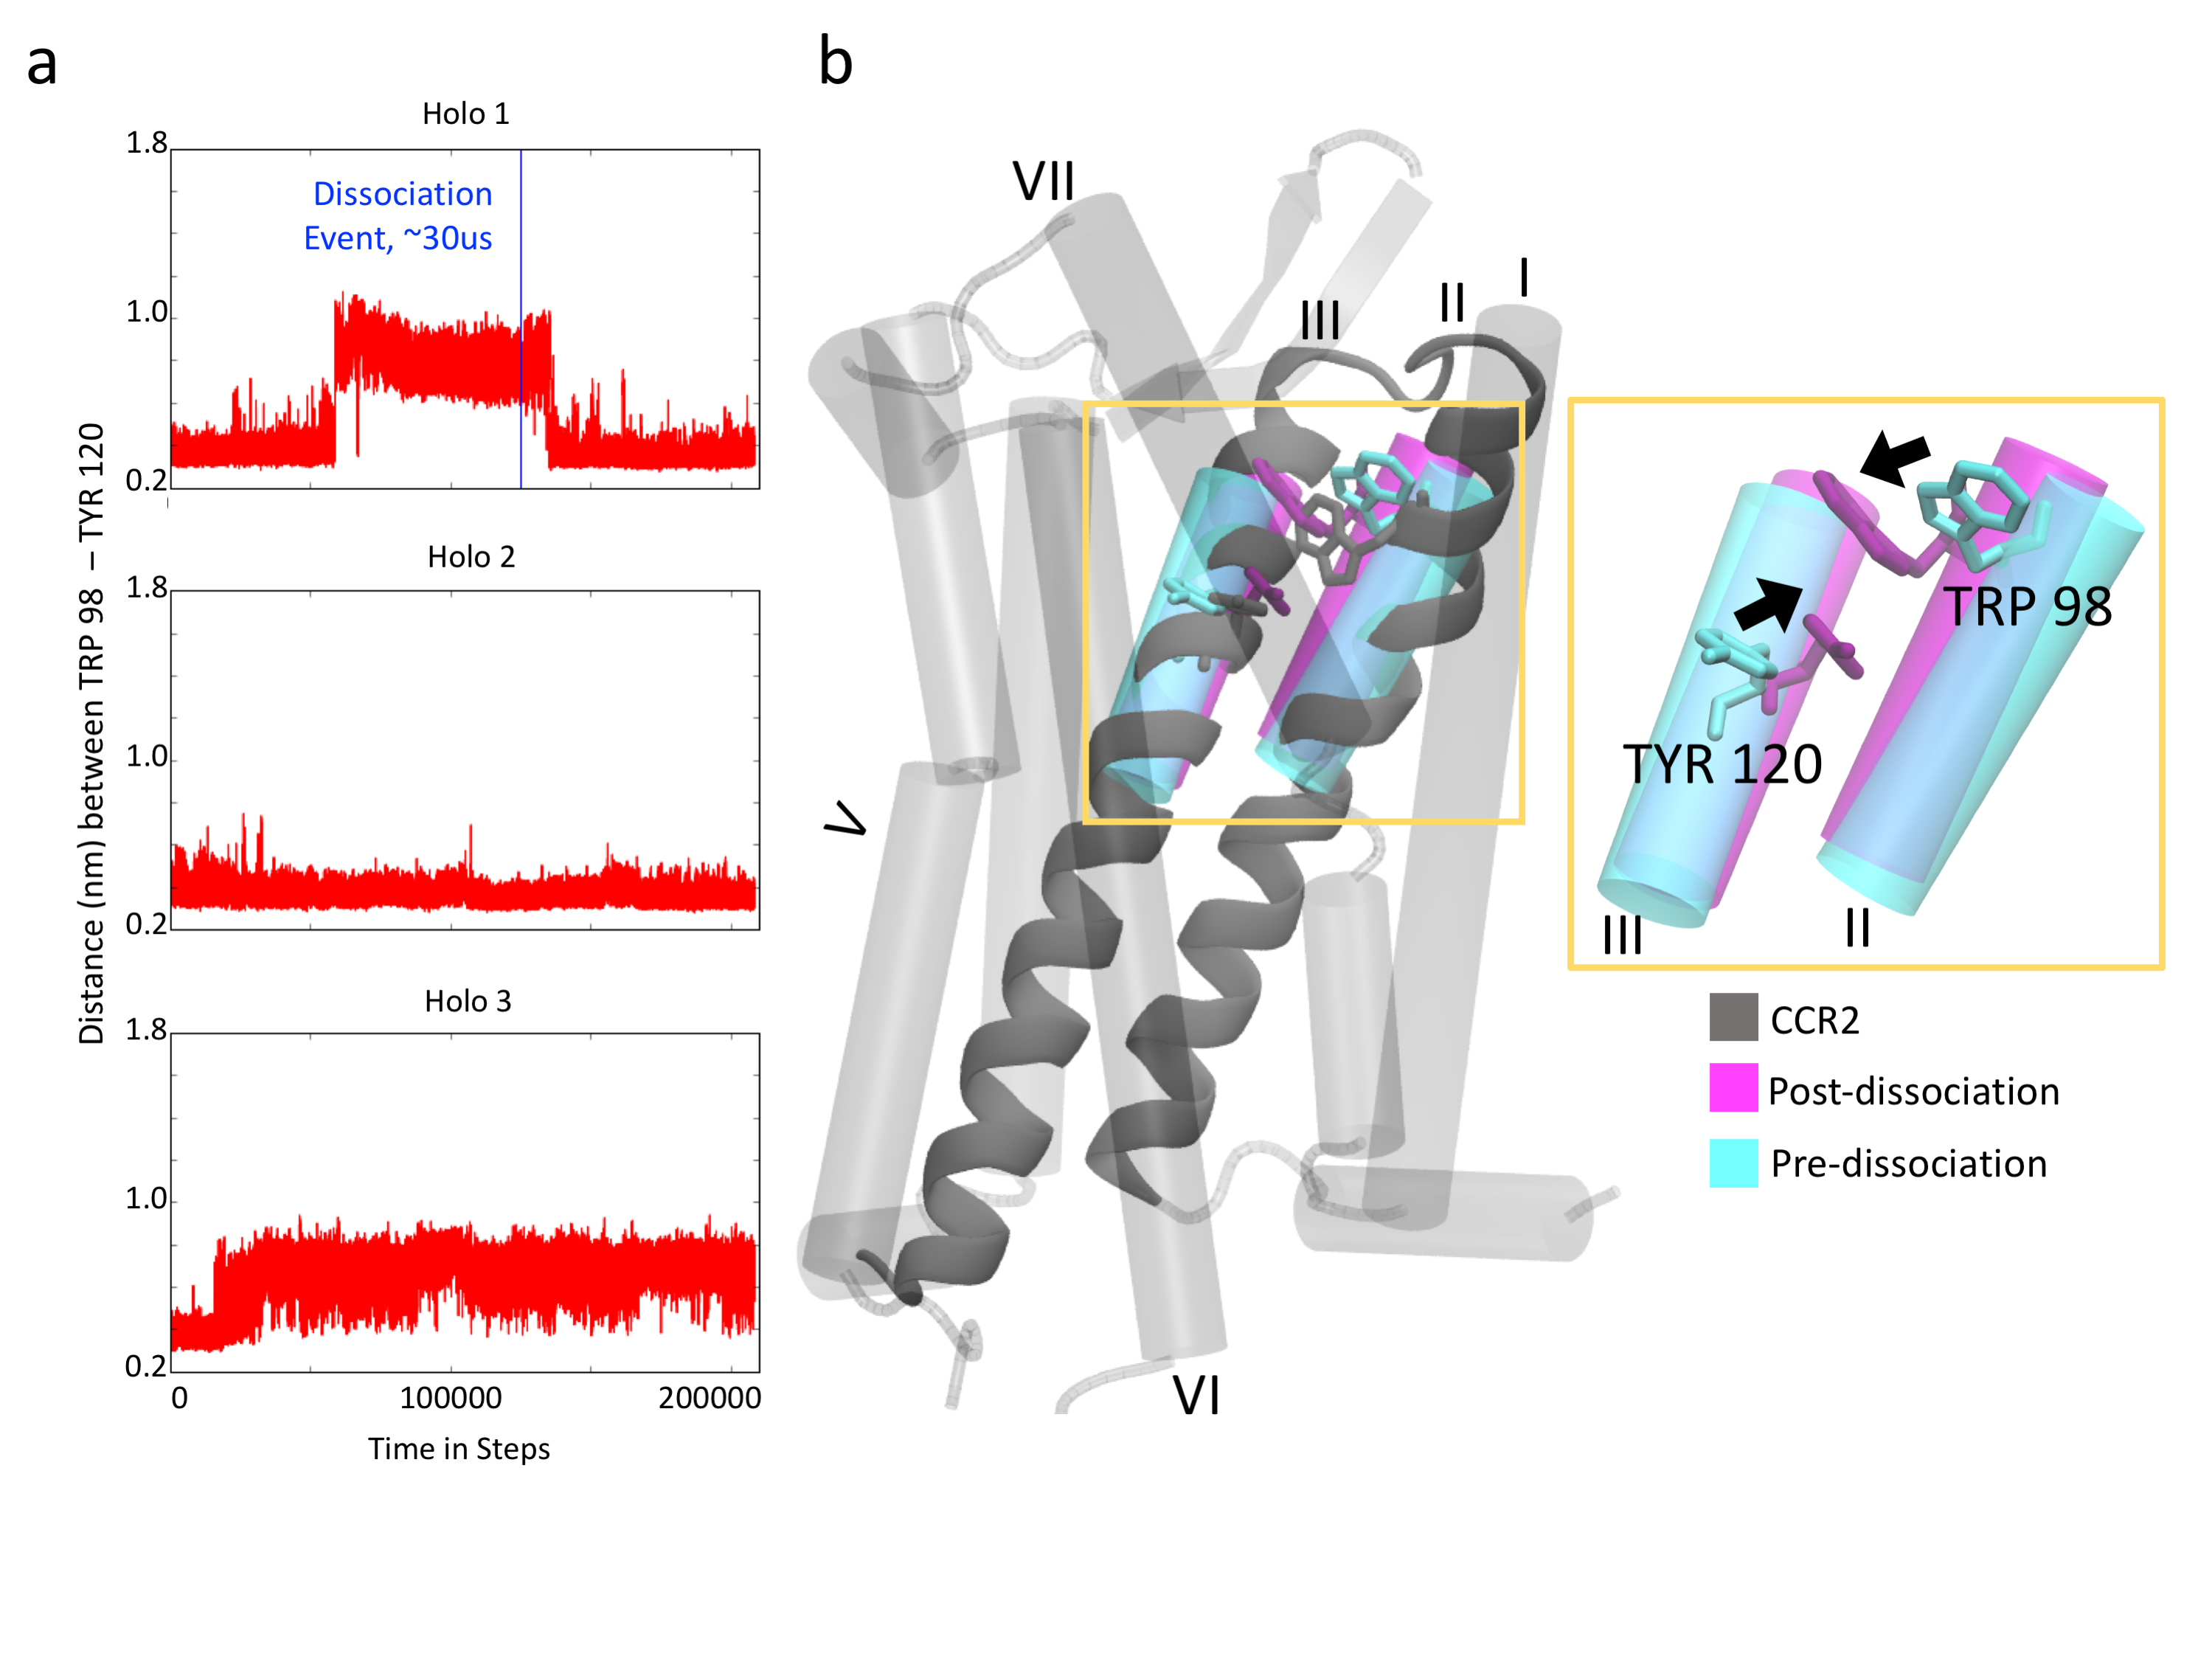
\includegraphics[width=\textwidth]{./figures/state35_98-120_larger.png}
 \caption{A) Distance between residues Trp 98\textsuperscript{2.60} and Tyr 120\textsuperscript{3.32} over simulation time. Dissociation event noted by blue line. B) Conformation of CCR2 before (teal) and after (purple) ligand dissociation.}
  \label{fig:state35_98-120}
\end{figure}

% glu 291 11
\begin{figure}[htbp]
  \centering
  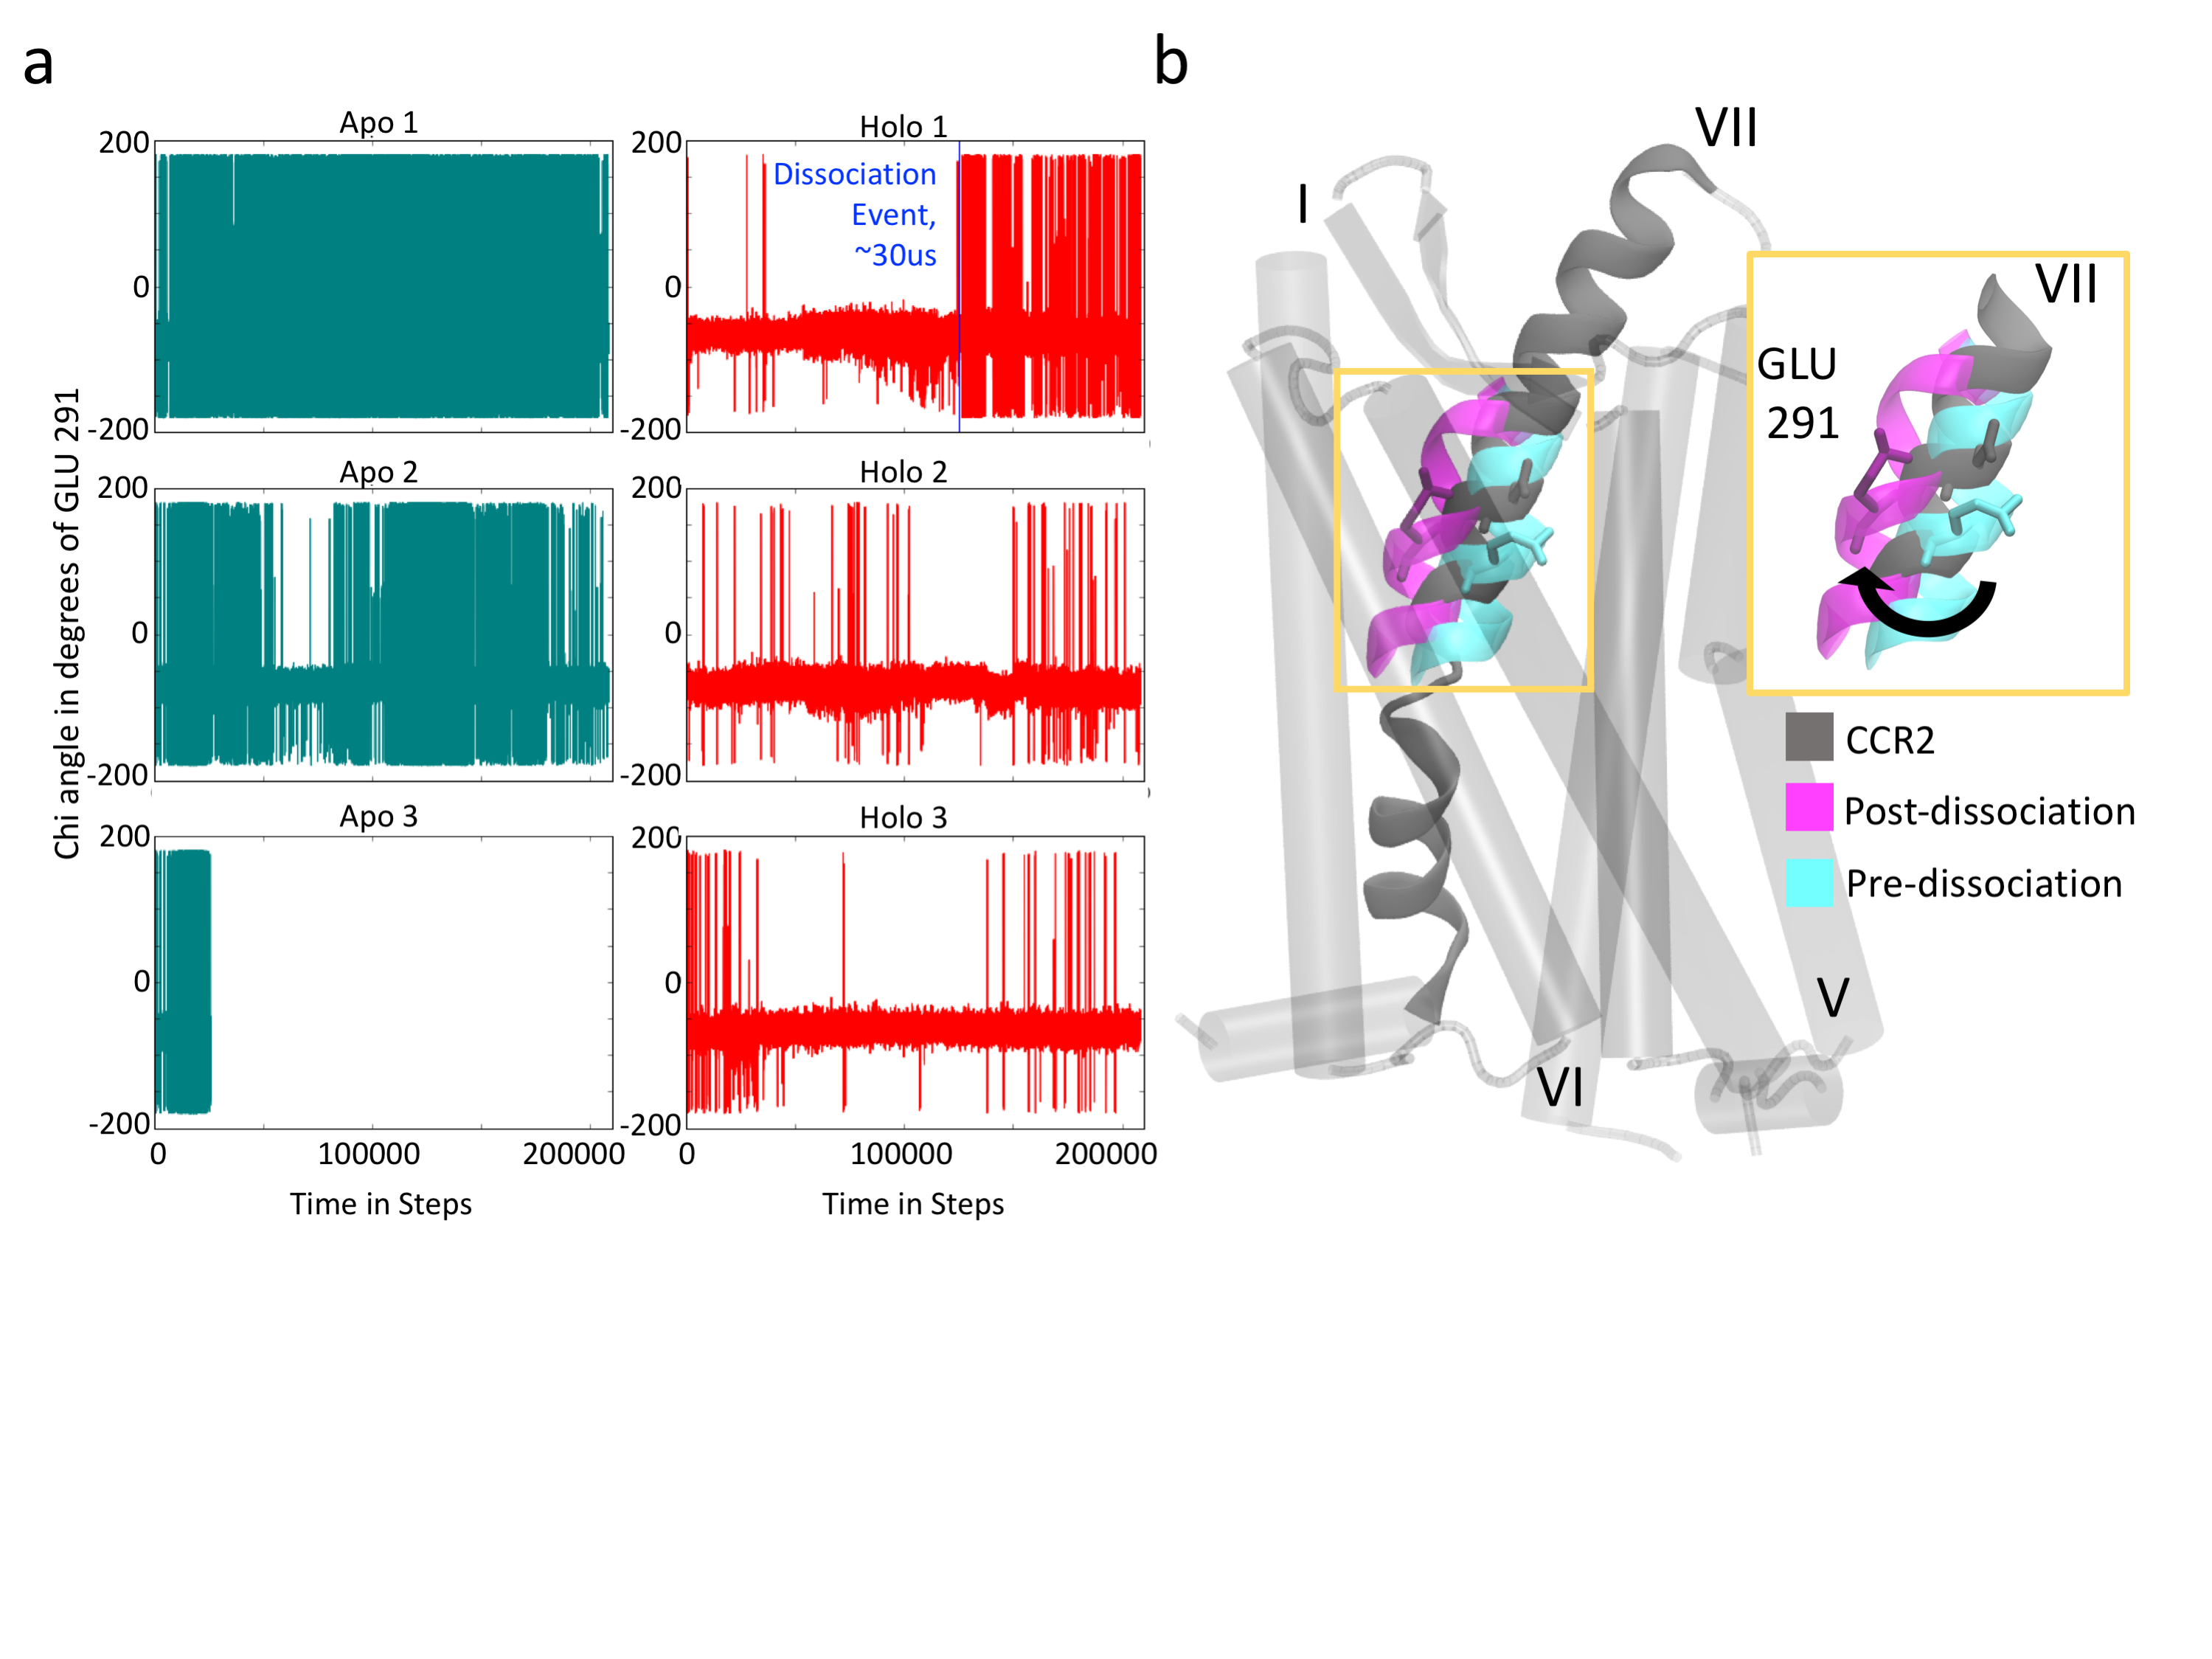
\includegraphics[width=\textwidth]{./figures/state35_glu291_larger.png}
 \caption{A) Chi angle of Glu 291 over simulation time. Dissociation event noted by blue line. B) Conformation of CCR2 before (teal) and after (purple) ligand dissociation.}
  \label{fig:state35_glu291}
\end{figure}

% 49-292 12
\begin{figure}[htbp]
  \centering
  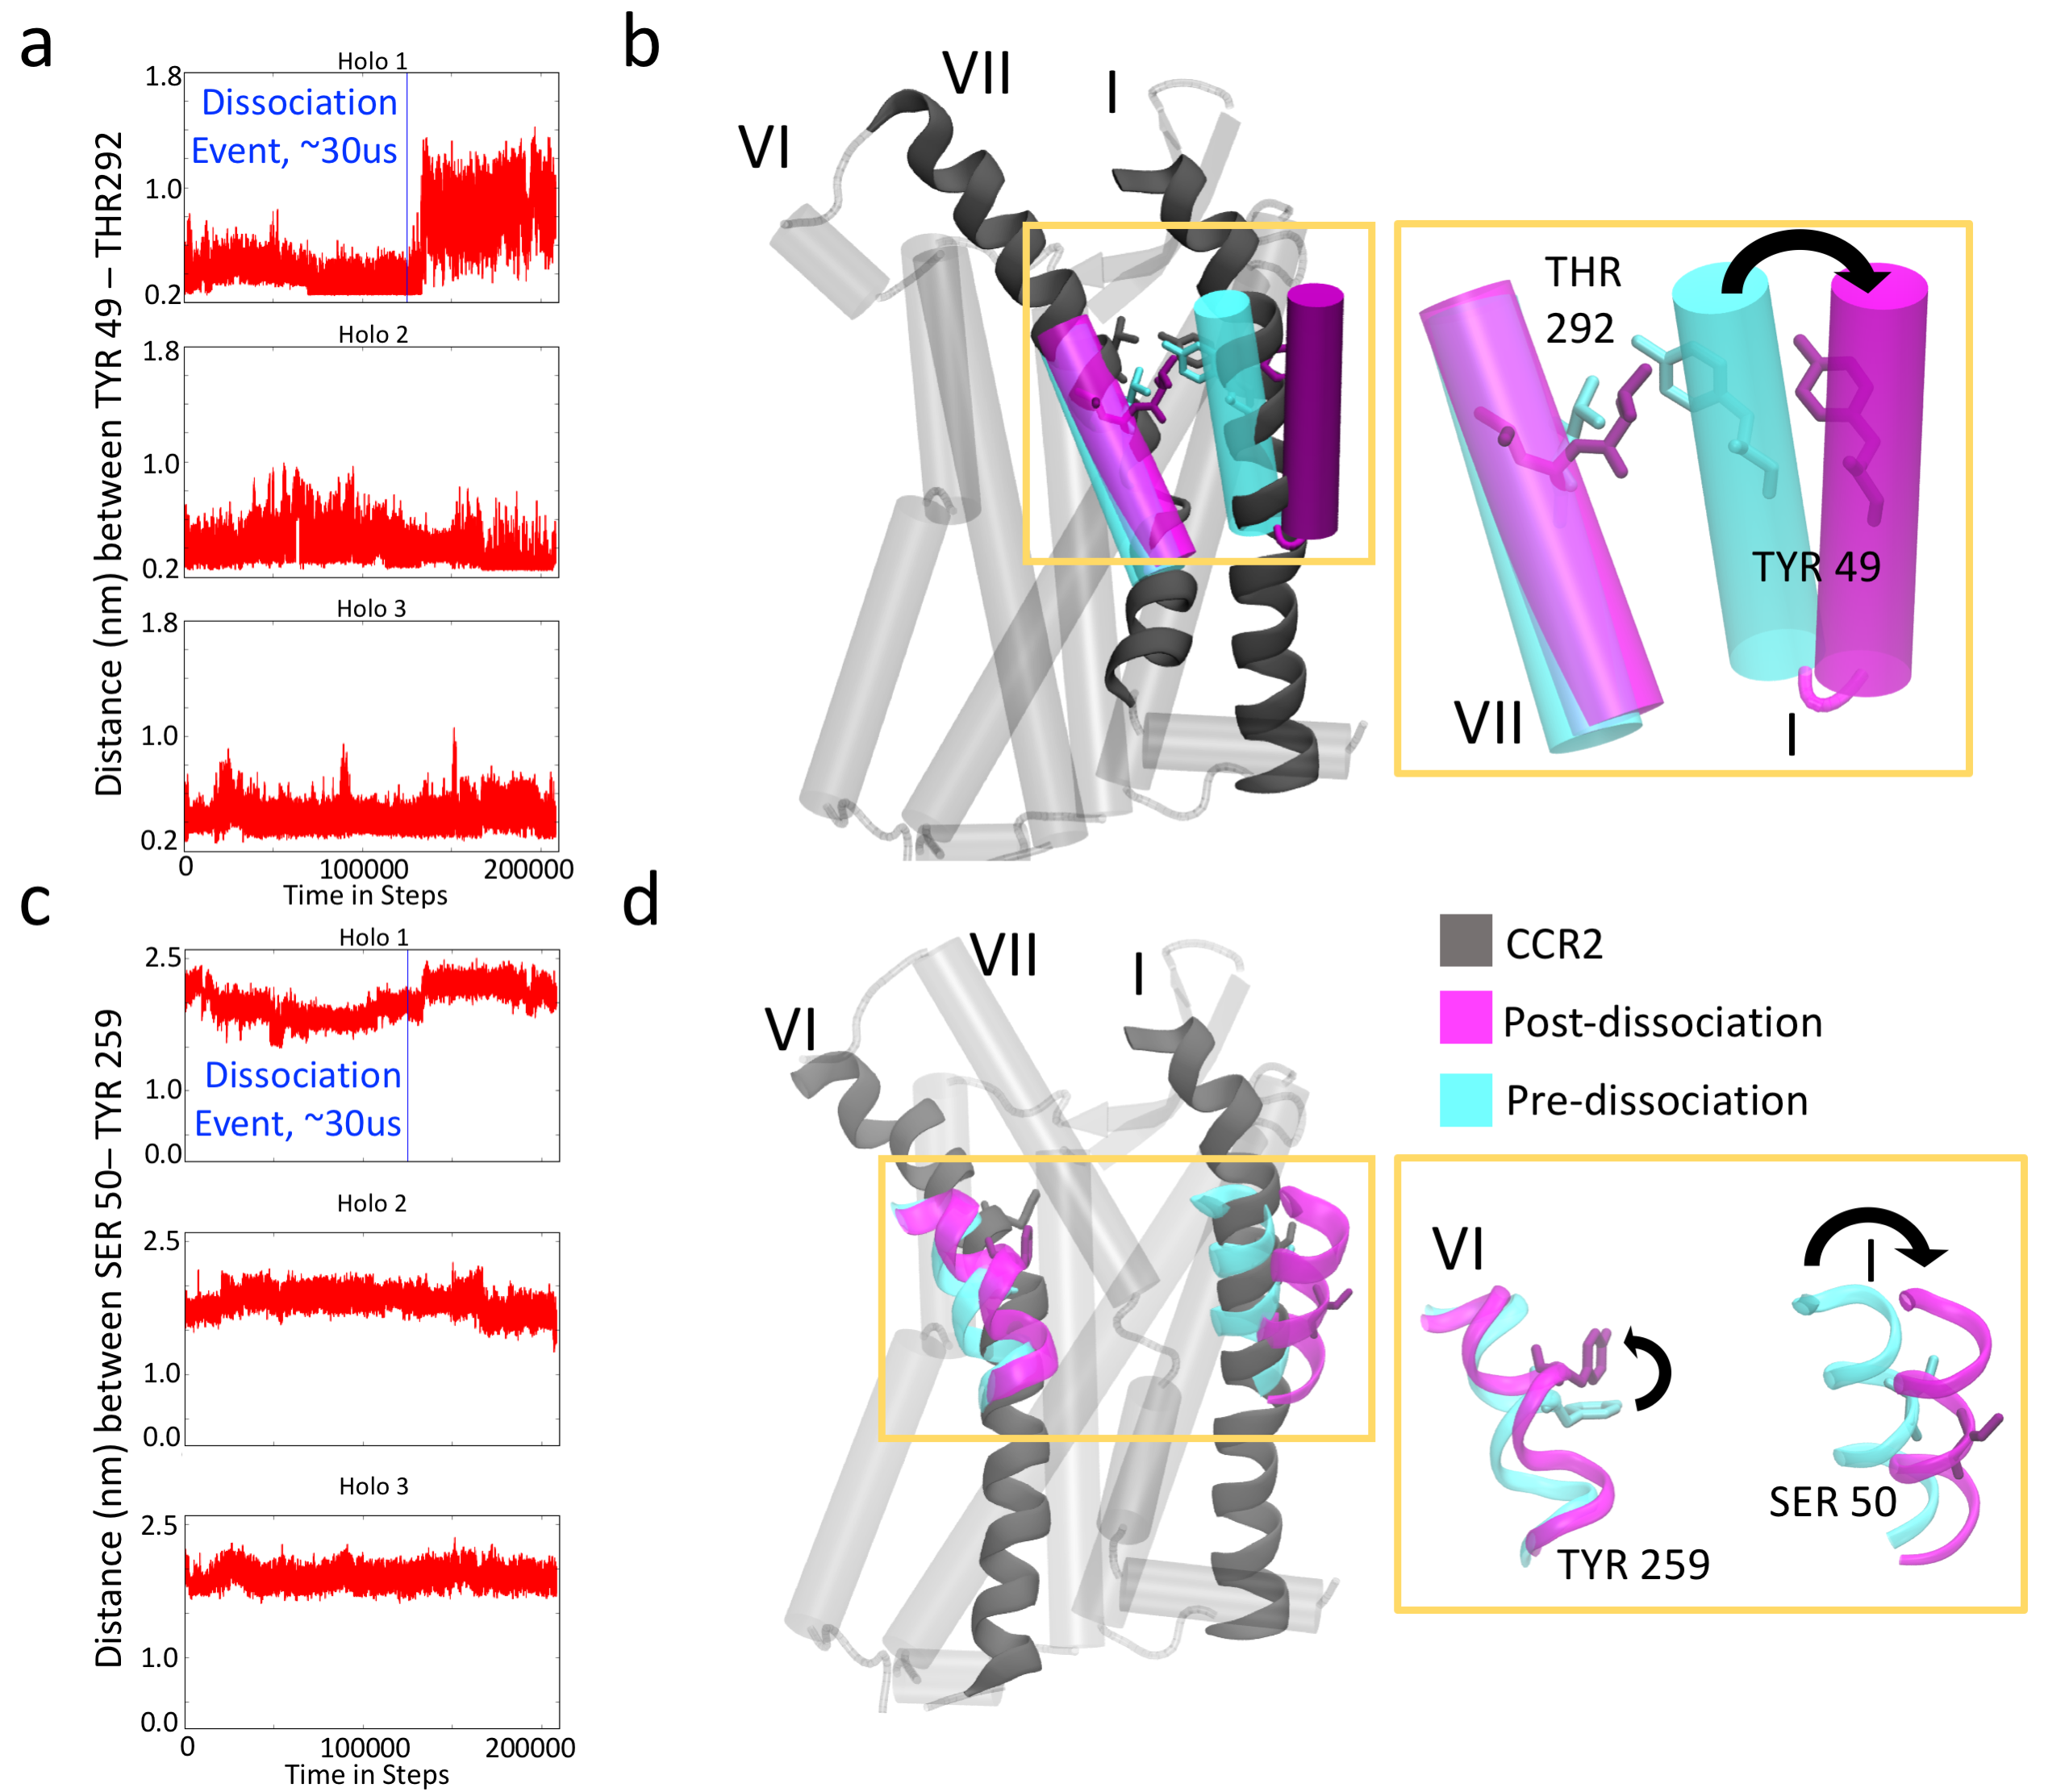
\includegraphics[width=\textwidth]{./figures/state35_49-292_50-259_larger.png}
 \caption{Orthosteric ligand dissociation breaks the hydrogen bond between key ligand binding residues. A) Distance between residues TYR 49\textsuperscript{1.39} - Thr 292 over simulation time. Dissociation event noted by blue line. B) Conformation of CCR2 before (teal) and after (purple) ligand dissociation. C) The distance between Ser 50\textsuperscript{1.40} and Tyr 259\textsuperscript{6.51} over simulation time. This distance is also a contributor to holo TIC 1, and shows the same outward movement of helix I. There is a slight decrease in distance between the residue pair, followed by the same lag time of 3 $\mu$s, and finally an increase in distance as the extracellular end of helix I bends away from the helical bundle. D) Conformation of CCR2 before (teal) and after (purple) ligand dissociation.}
  \label{fig:state35_49-292_50-259}
\end{figure}

% RMSF / SASA 13
\begin{figure}[htbp]
  \centering
  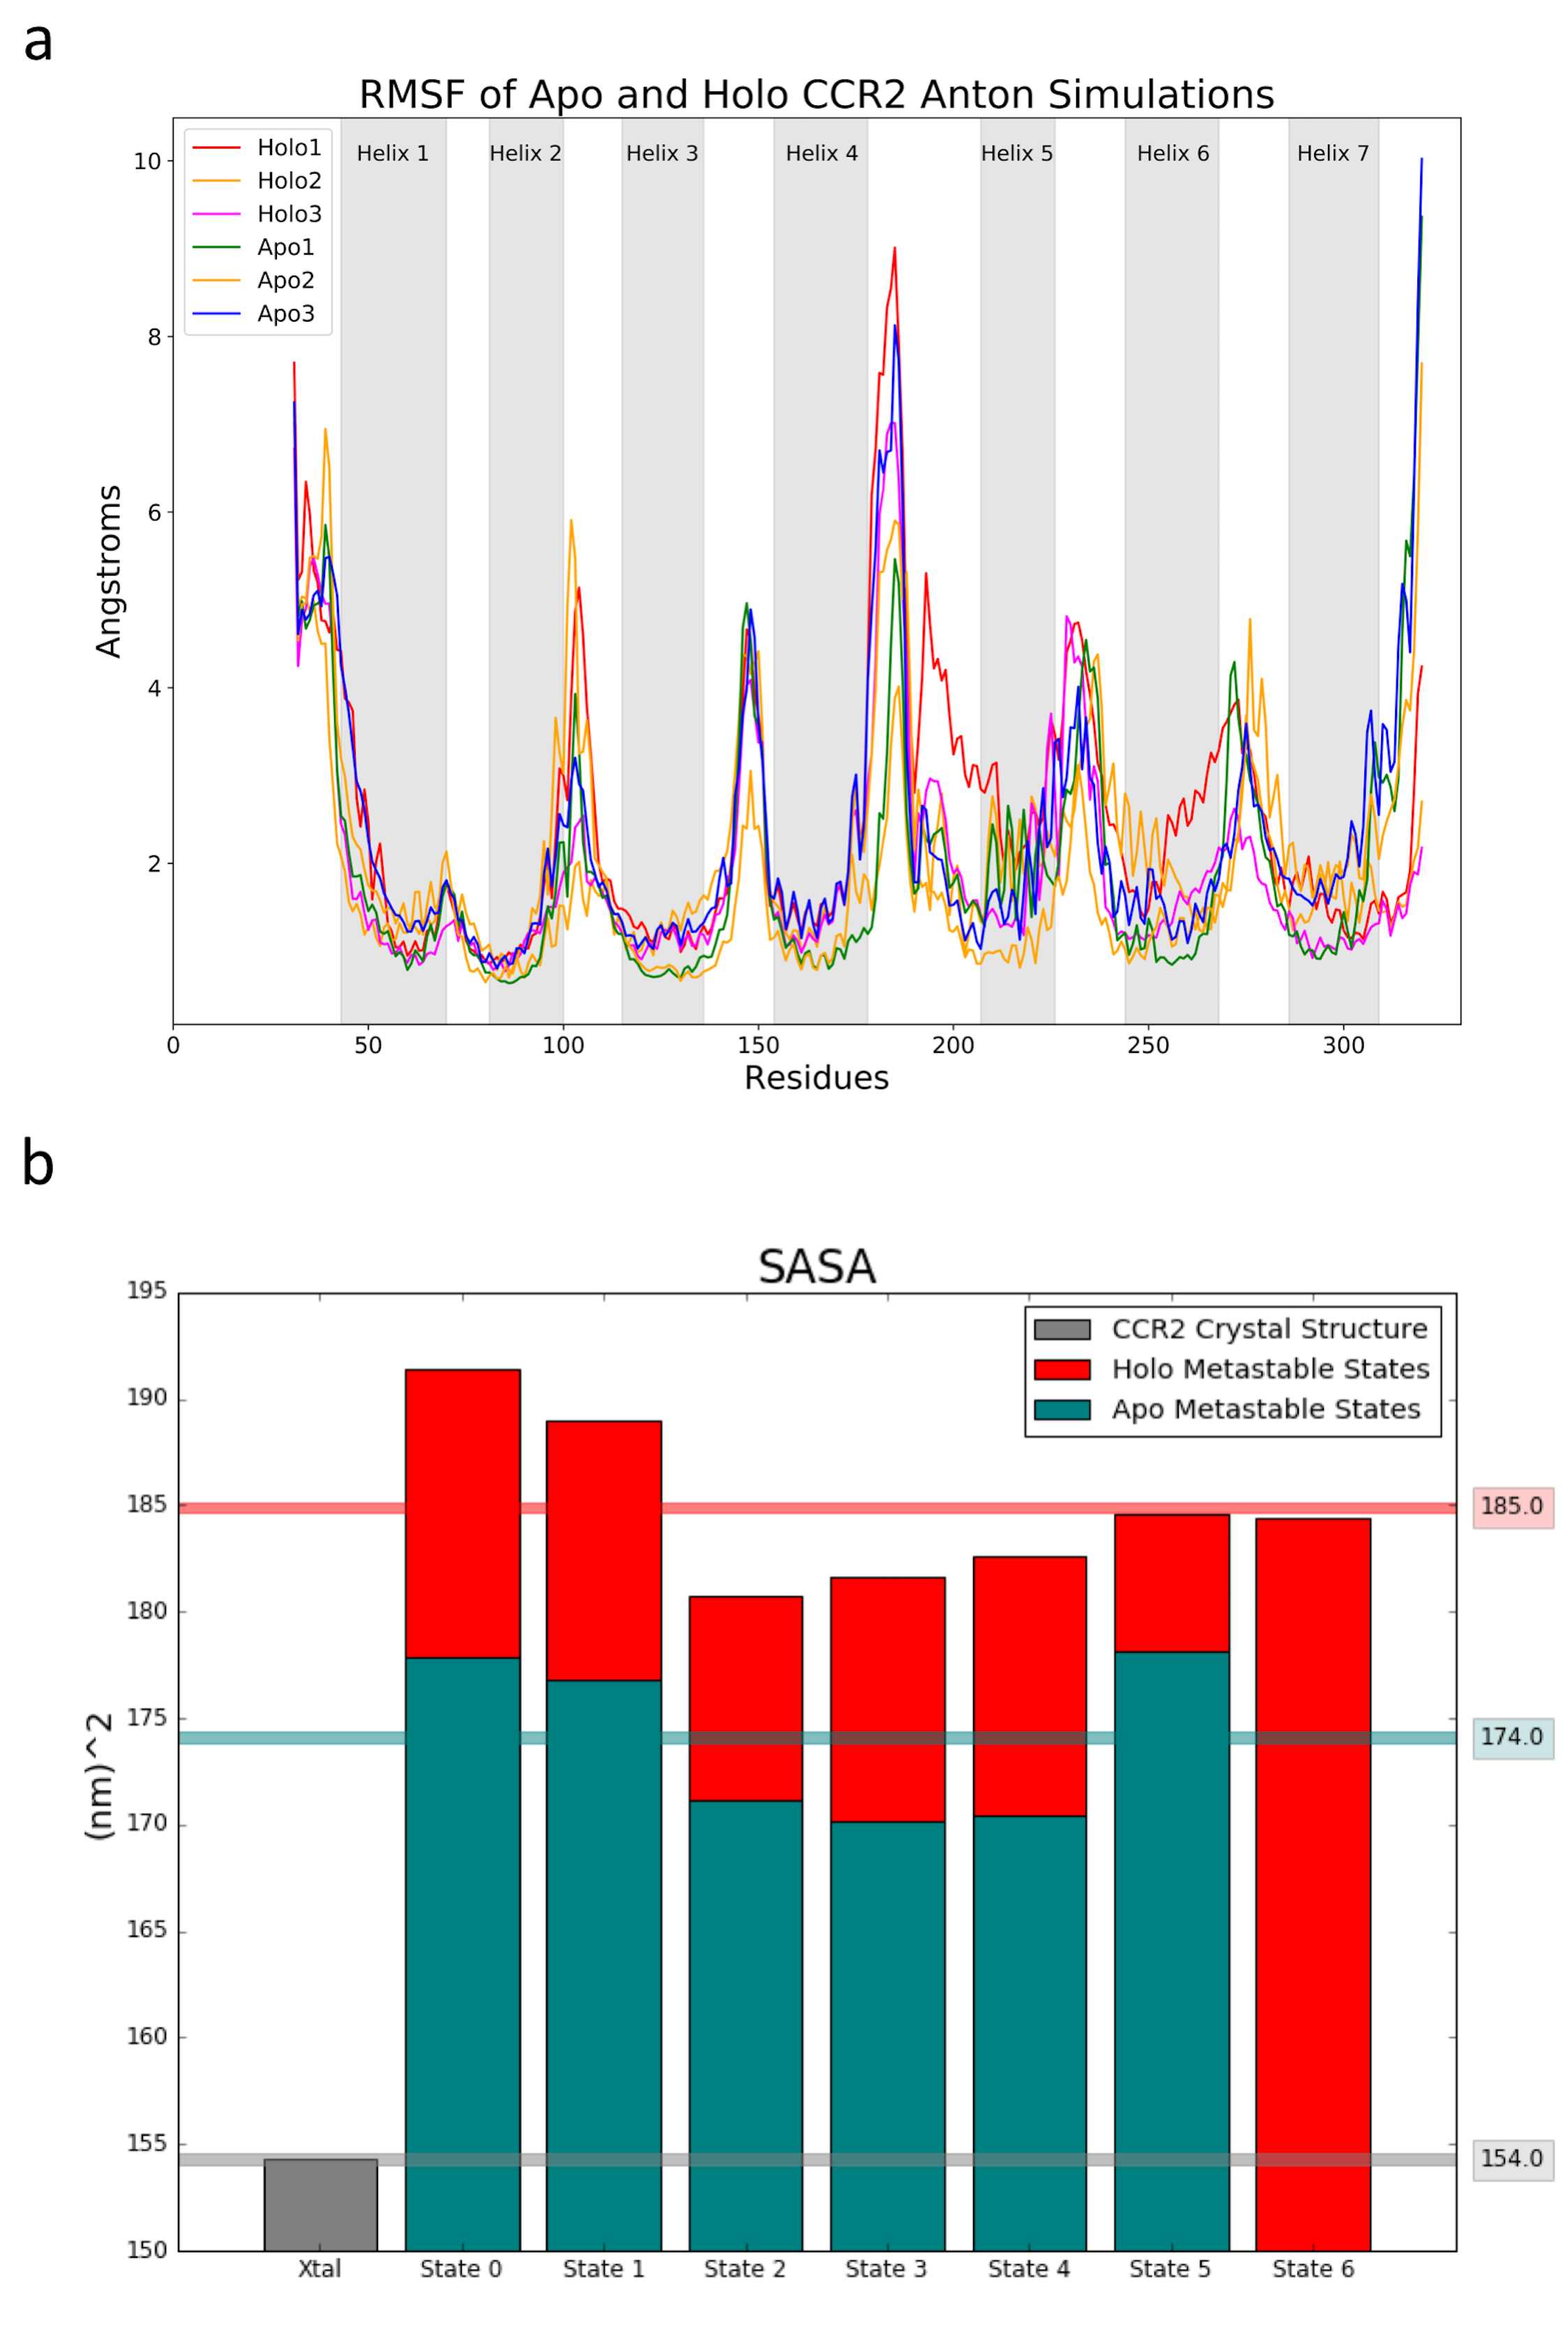
\includegraphics[width=\textwidth,height=0.9\textheight,keepaspectratio]{./figures/rmsf_sasa.png}
 \caption{A) RMSF of each residue for individual simulations of apo and holo CCR2. B) SASA for each metastable macrostate of apo and holo, compared to the CCR2 crystal structure.}
  \label{fig:rmsf_sasa}
\end{figure}

% ITS 14
\begin{figure}[htbp]
\centering
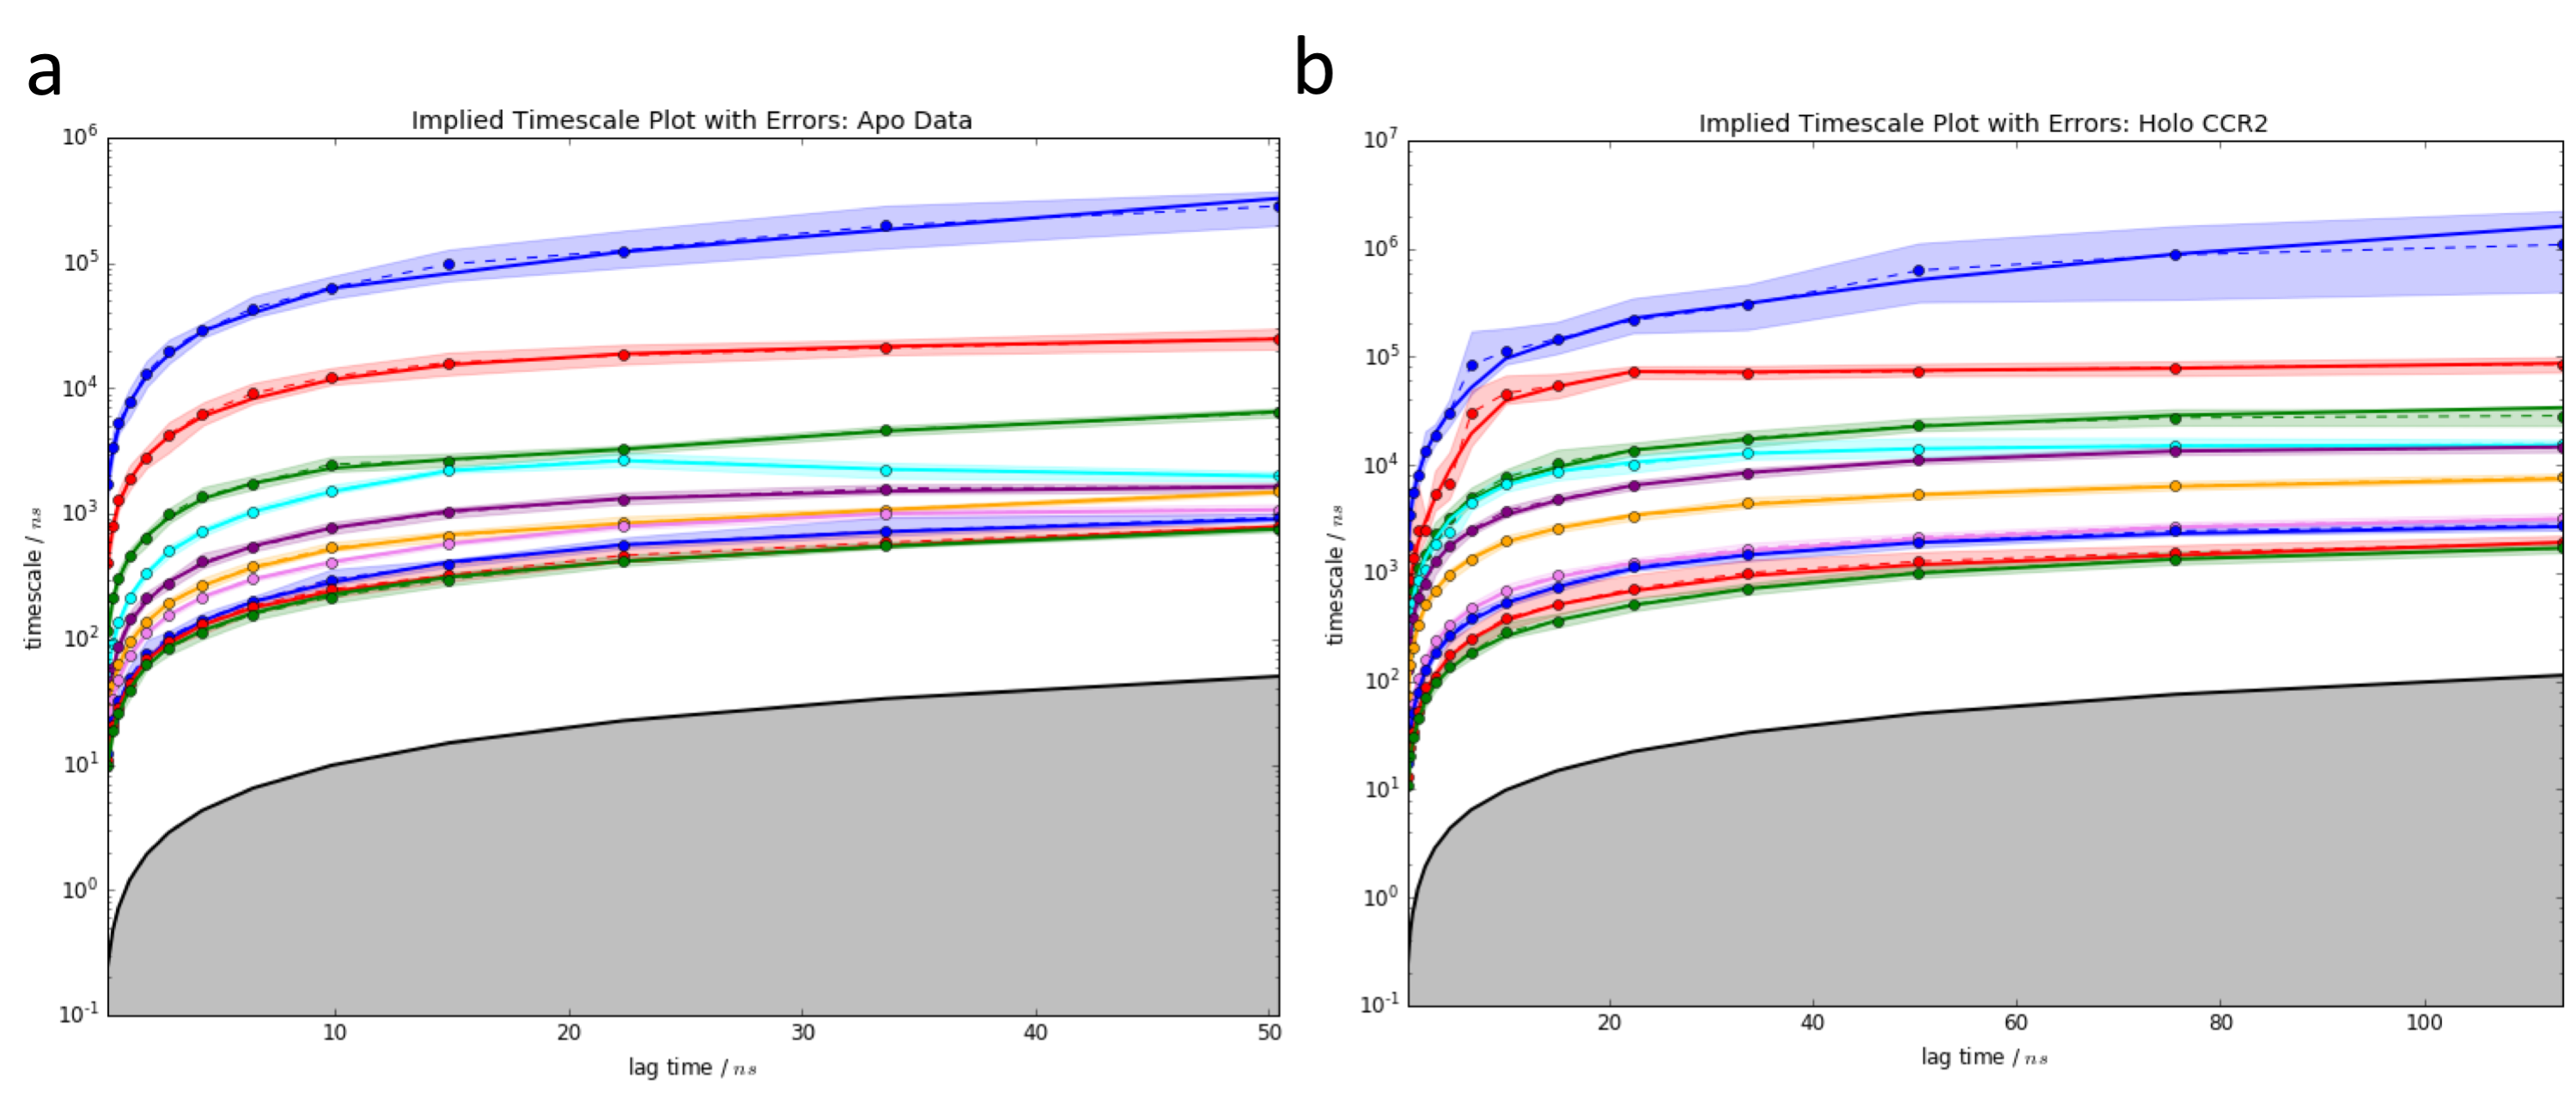
\includegraphics[width=\textwidth]{./figures/its.png}
\caption{Implied timescale plots for A) apo and B) holo CCR2.}
\label{fig:its}
\end{figure}

% CK apo 15
\begin{figure}[htbp]
\centering
\includegraphics[width=\textwidth]{./figures/apo_cktest_largefont.png}
\caption{CK Test for apo CCR2.}
\label{fig:apo_its_ck}
\end{figure}

% CK holo 16
\begin{figure}[htbp]
  \centering
  \includegraphics[width=\textwidth]{./figures/holo_cktest_largefont.png}
 \caption{CK Test for holo CCR2}
  \label{fig:holo_its_ck}
\end{figure}

%Centroid Figures 17
\begin{figure}[htbp]
\centering
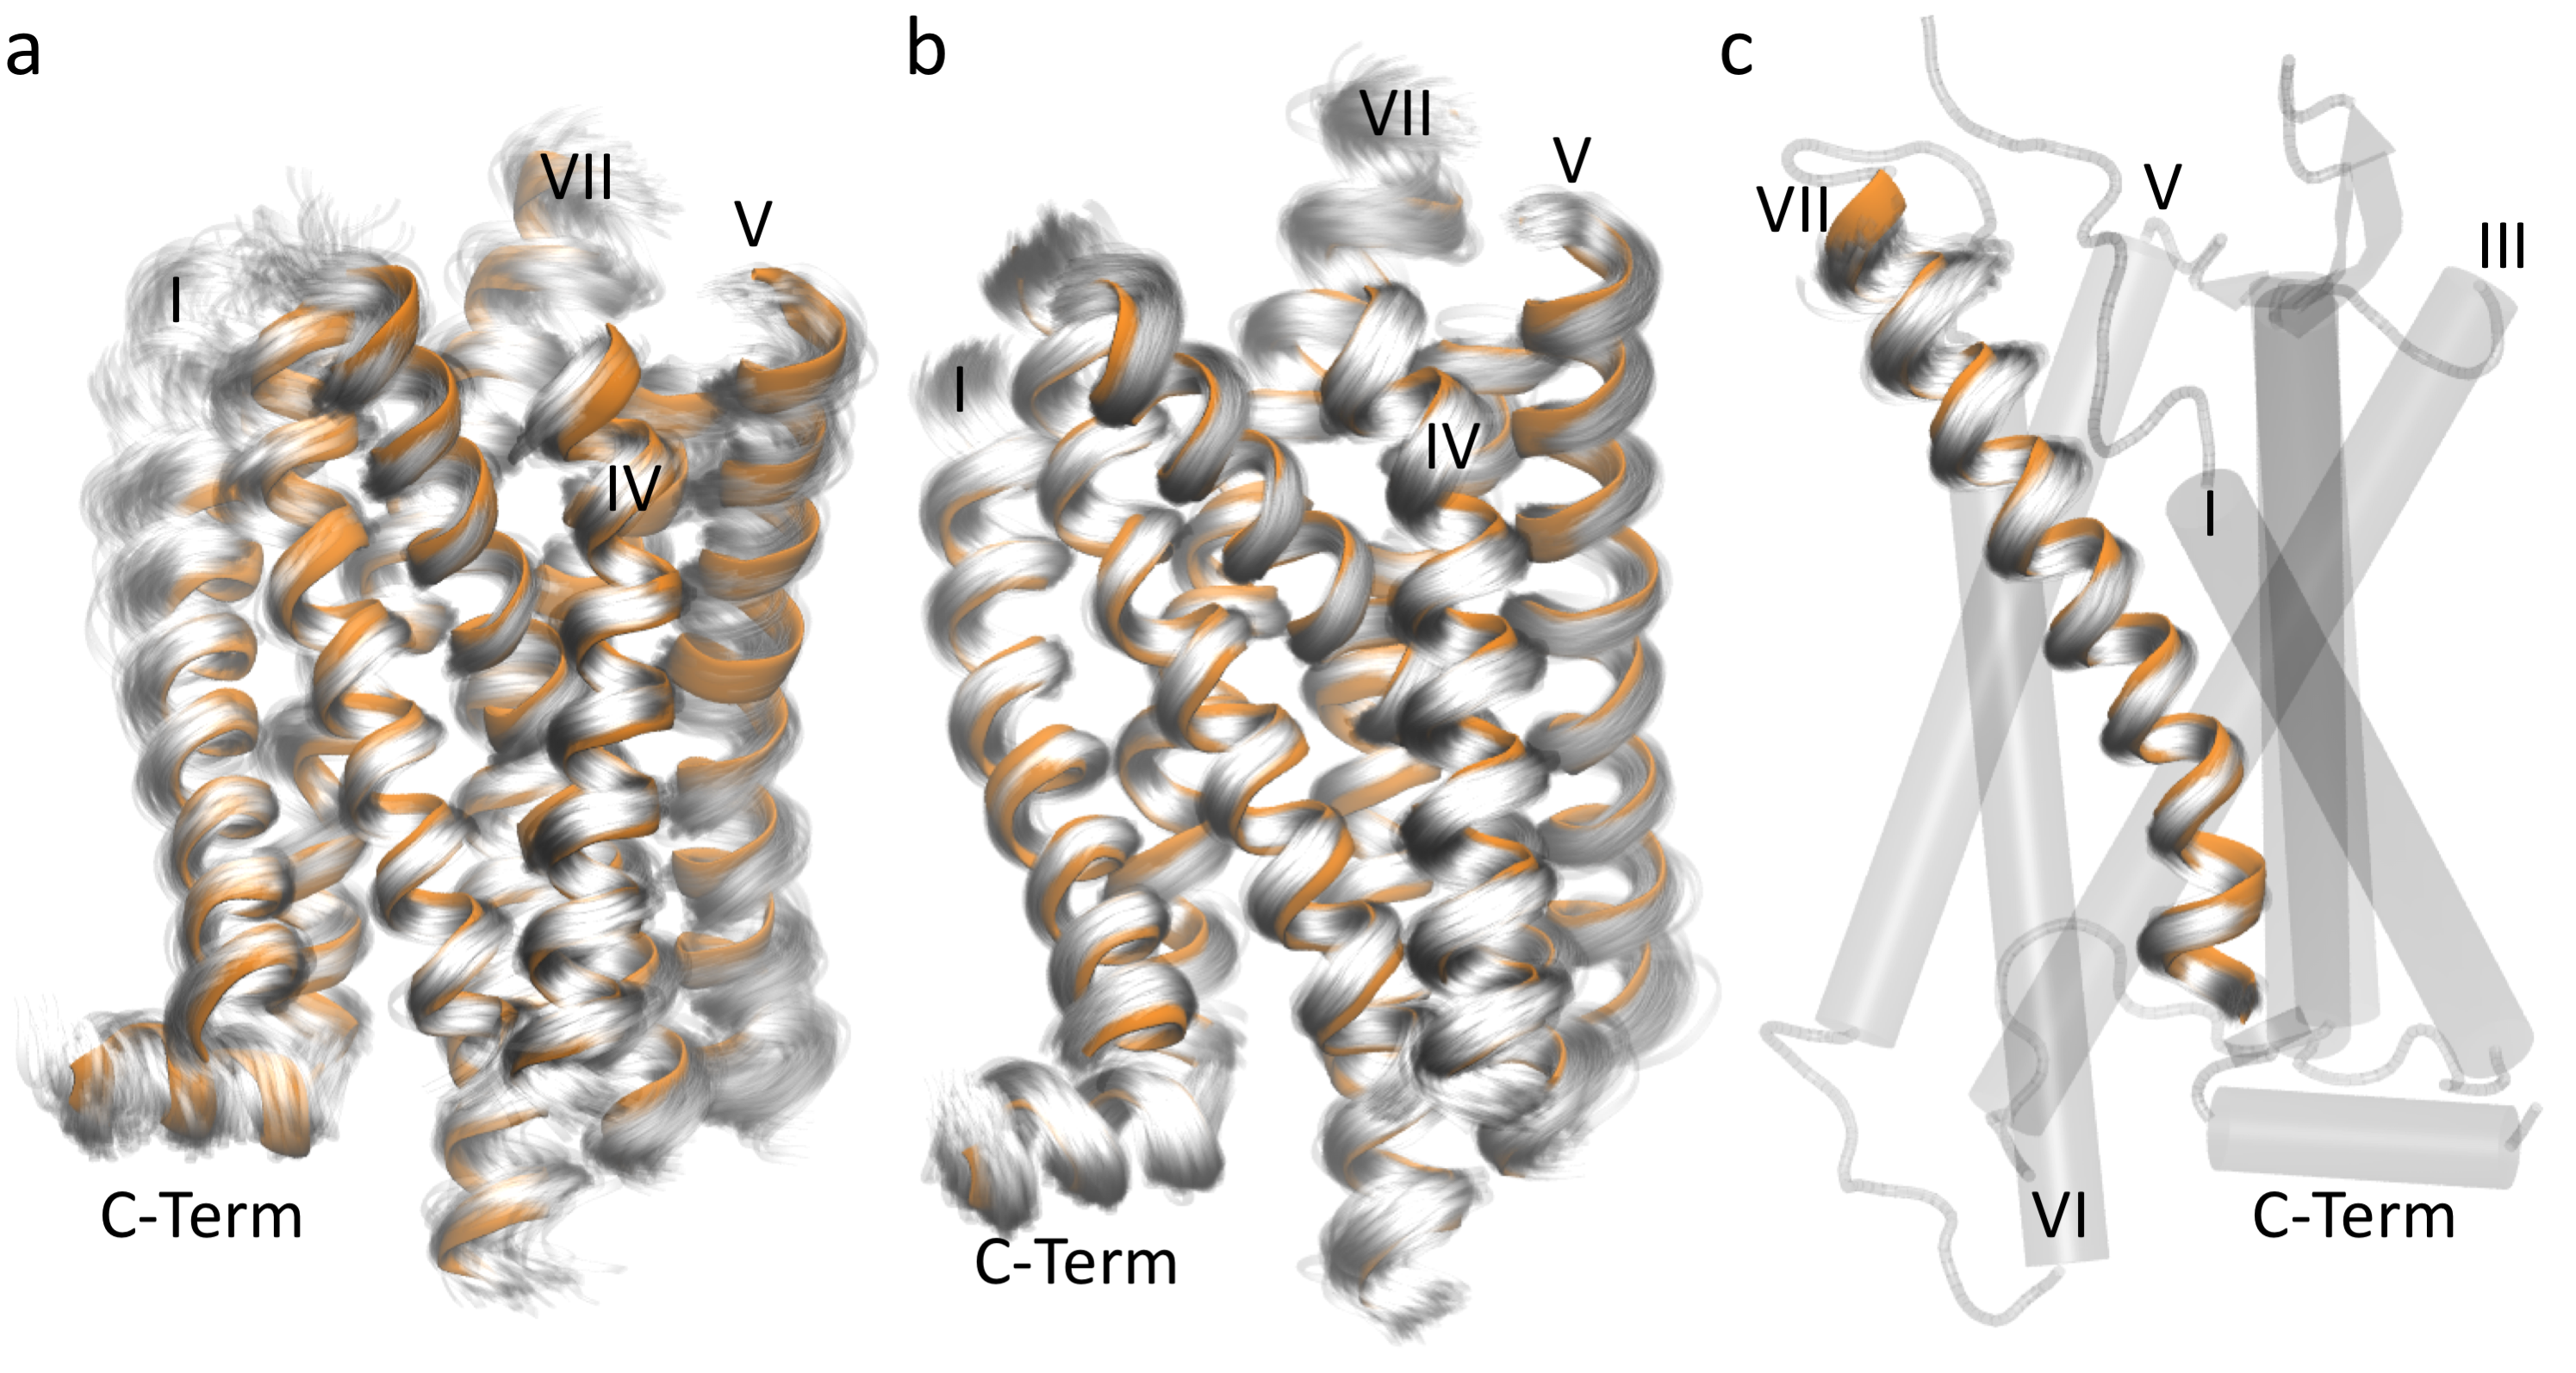
\includegraphics[width=\textwidth]{./figures/centroid-micromacrostates.png}
\caption{The centroid of apo macrostate A, in orange, is compared to A) the 214 other microstate centroids in white (average RMSD of alpha helices from representative structure: 2.01 {\AA}, standard deviation 0.50 {\AA}), and B) the 1,024 frames from its microstate in white (average RMSD of alpha helices from centroid: 0.872 {\AA}, standard deviation 0.139 {\AA}). C) Helix VII of the same microstate (average RMSD from centroid: 1.035 {\AA}, standard deviation 0.259 {\AA}.)}
\label{fig:centroid-helixVII}
\end{figure}

%Centroid Figures 18
\begin{figure}[htbp]
\centering
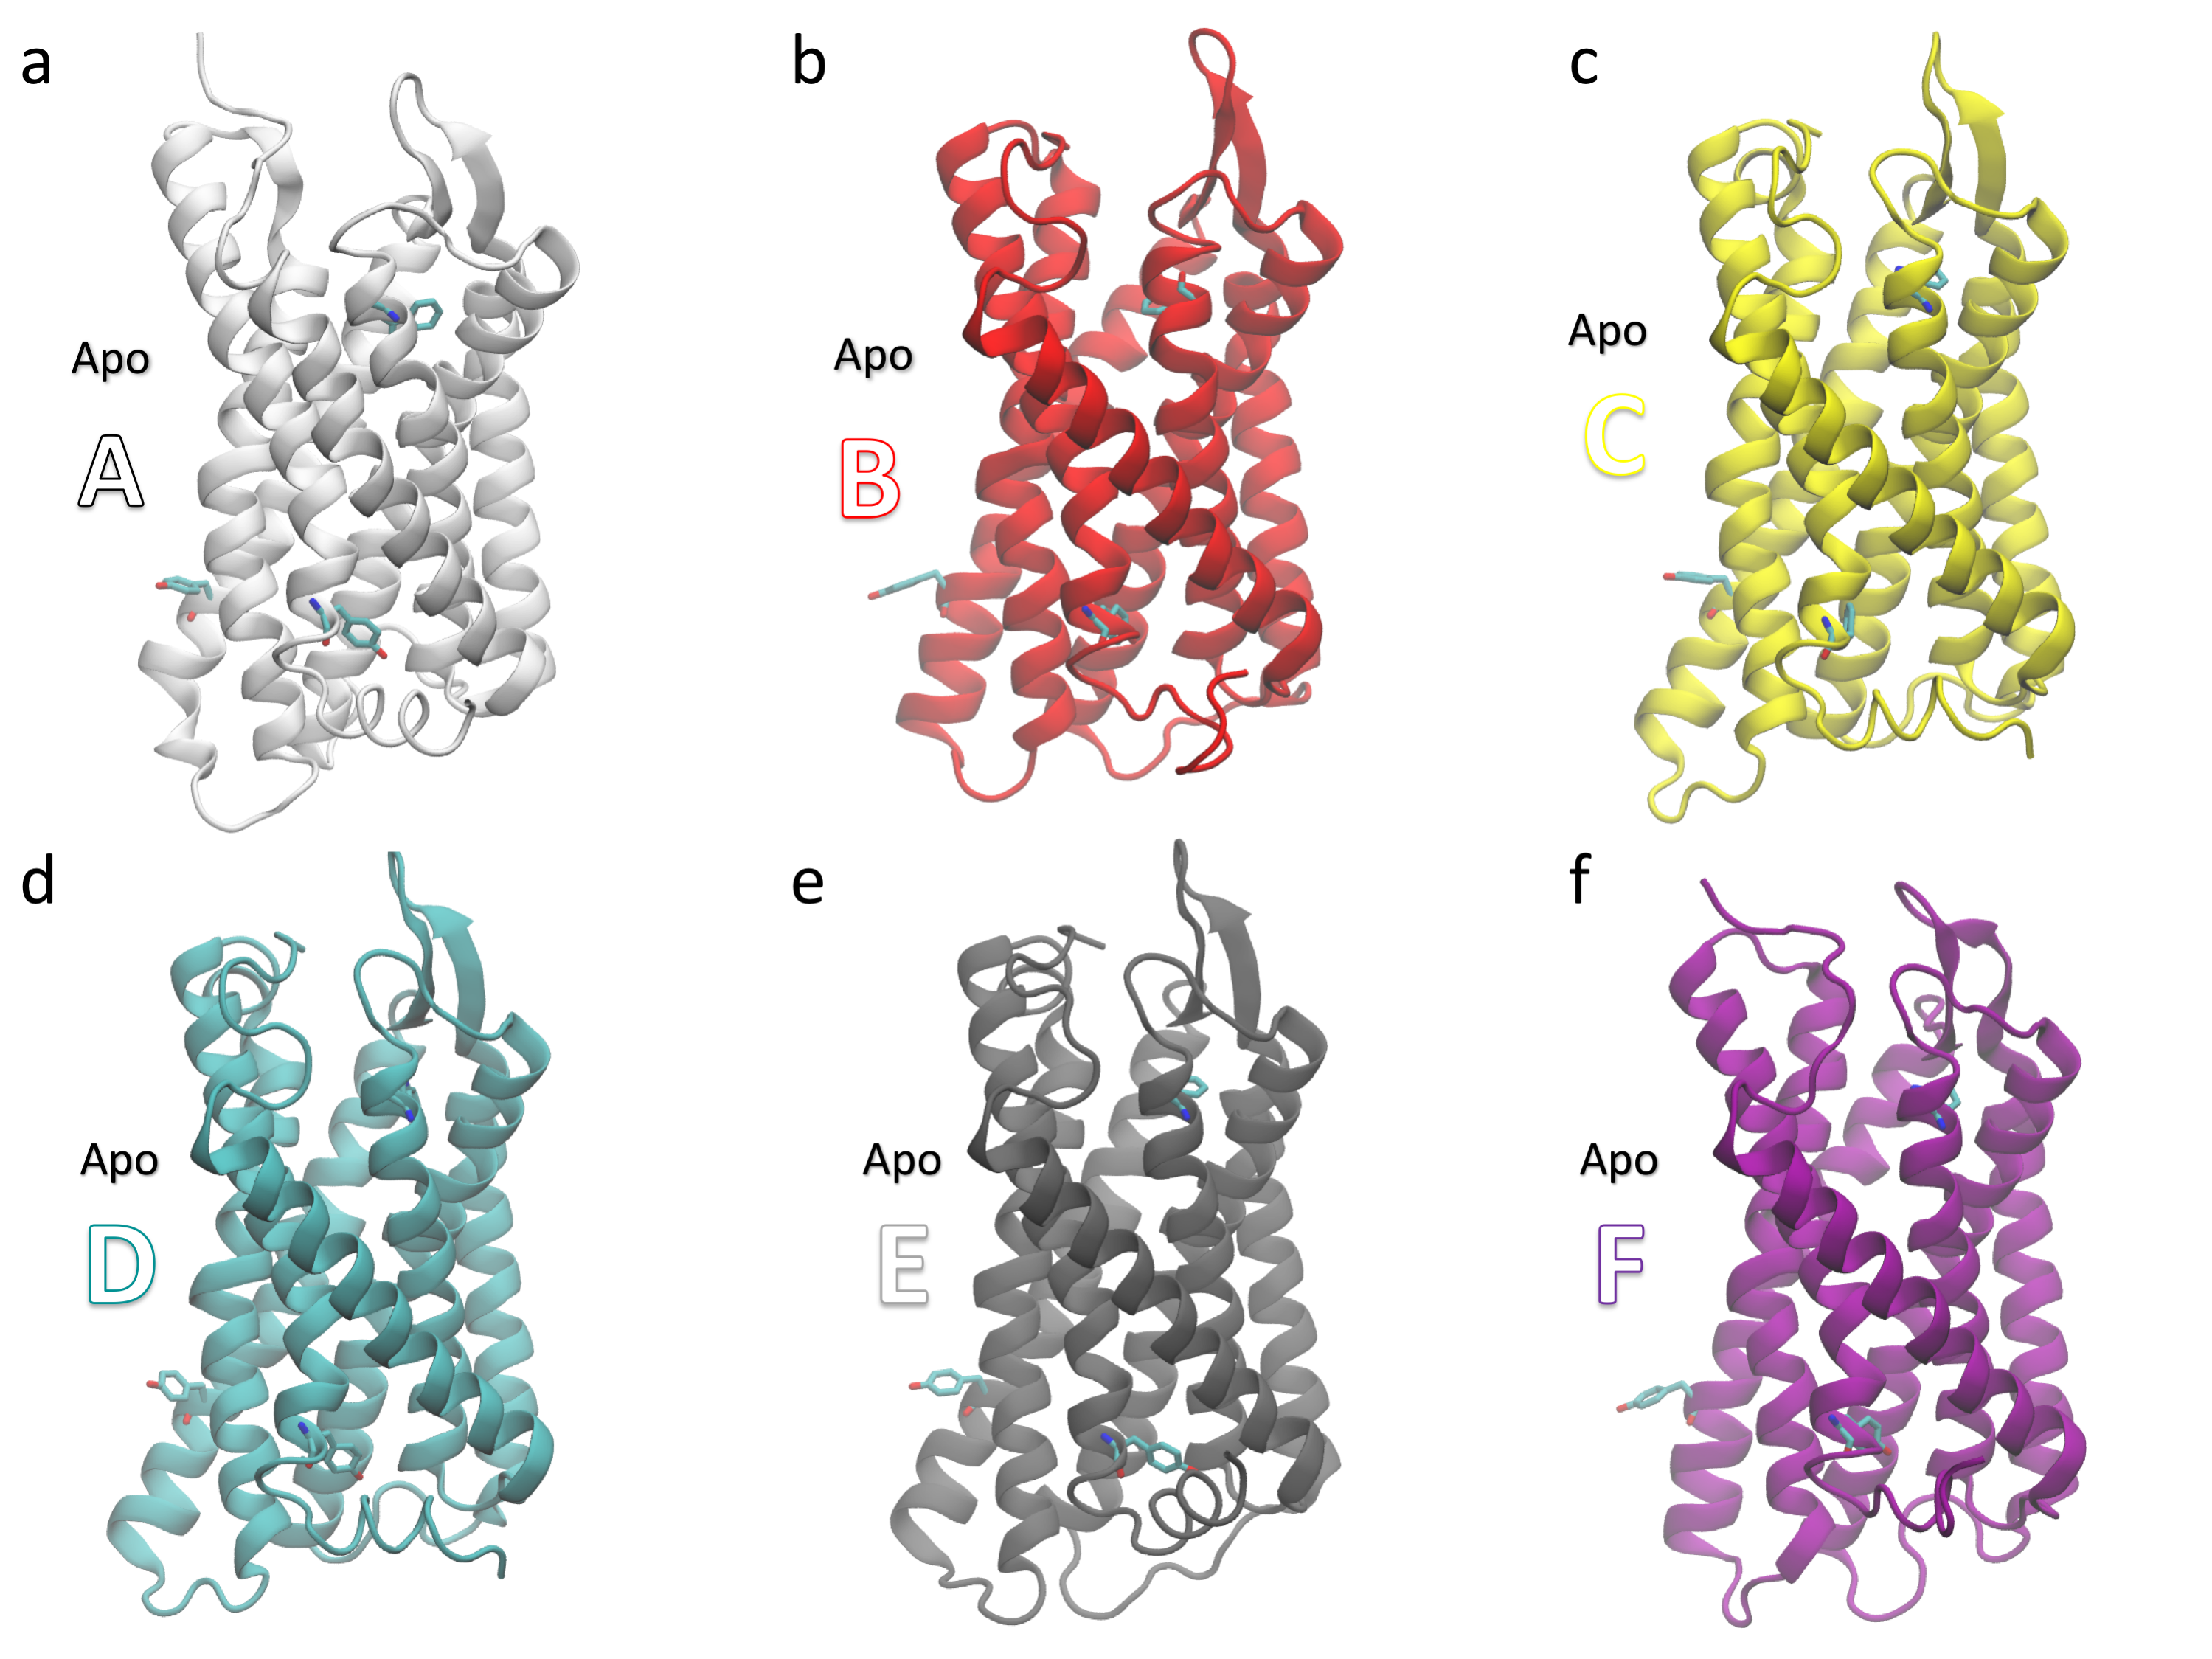
\includegraphics[width=\textwidth]{./figures/apo-centroids.png}
\caption{The apo macrostates.}
\label{fig:apo-centroids}
\end{figure}

%Centroid Figures 19
\begin{figure}[htbp]
\centering
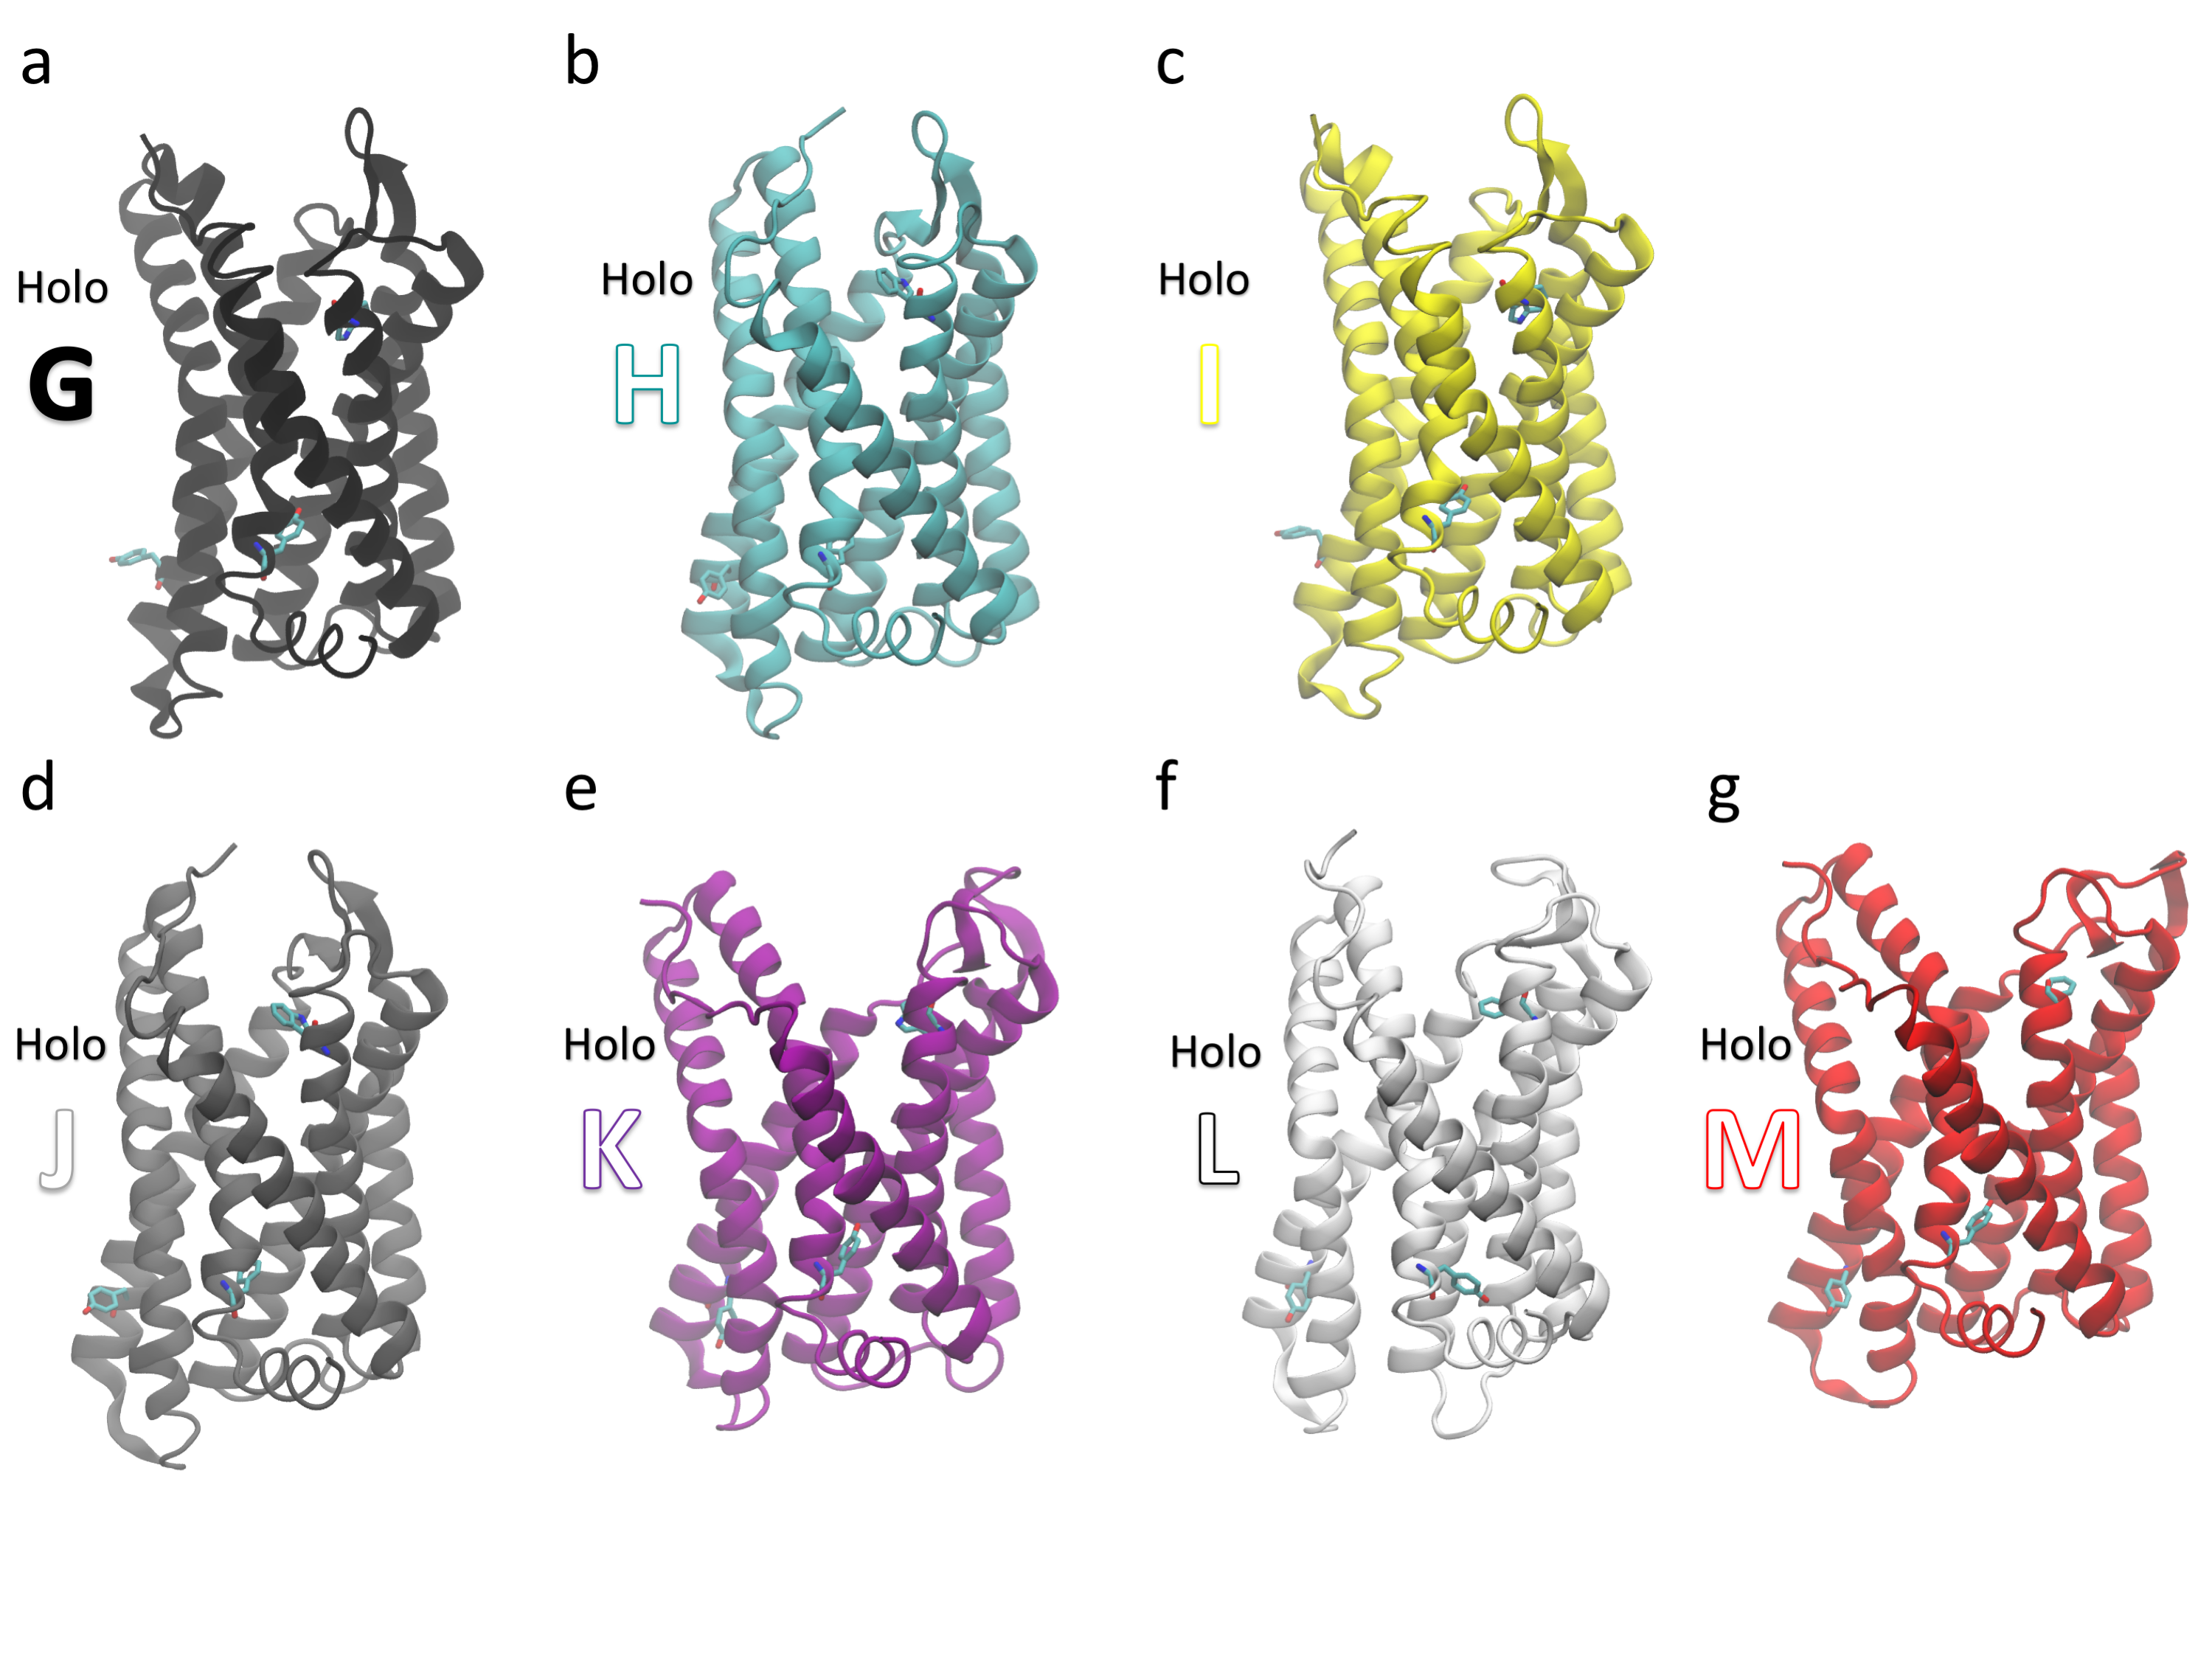
\includegraphics[width=\textwidth]{./figures/holo-centroids.png}
\caption{The holo macrostates.}
\label{fig:holo-centroids}
\end{figure}